	%!TEX root = ../template.tex
%%%%%%%%%%%%%%%%%%%%%%%%%%%%%%%%%%%%%%%%%%%%%%%%%%%%%%%%%%%%%%%%%%%%
%% chapter4.tex
%% NOVA thesis document file
%%
%% Chapter with lots of dummy text
%%%%%%%%%%%%%%%%%%%%%%%%%%%%%%%%%%%%%%%%%%%%%%%%%%%%%%%%%%%%%%%%%%%%

\typeout{NT FILE chapter4.tex}%

\chapter{Unveiling the \textit{Grammar} of Time Series}
\label{cha:segmentation}

\begin{figure}[h]
\centering
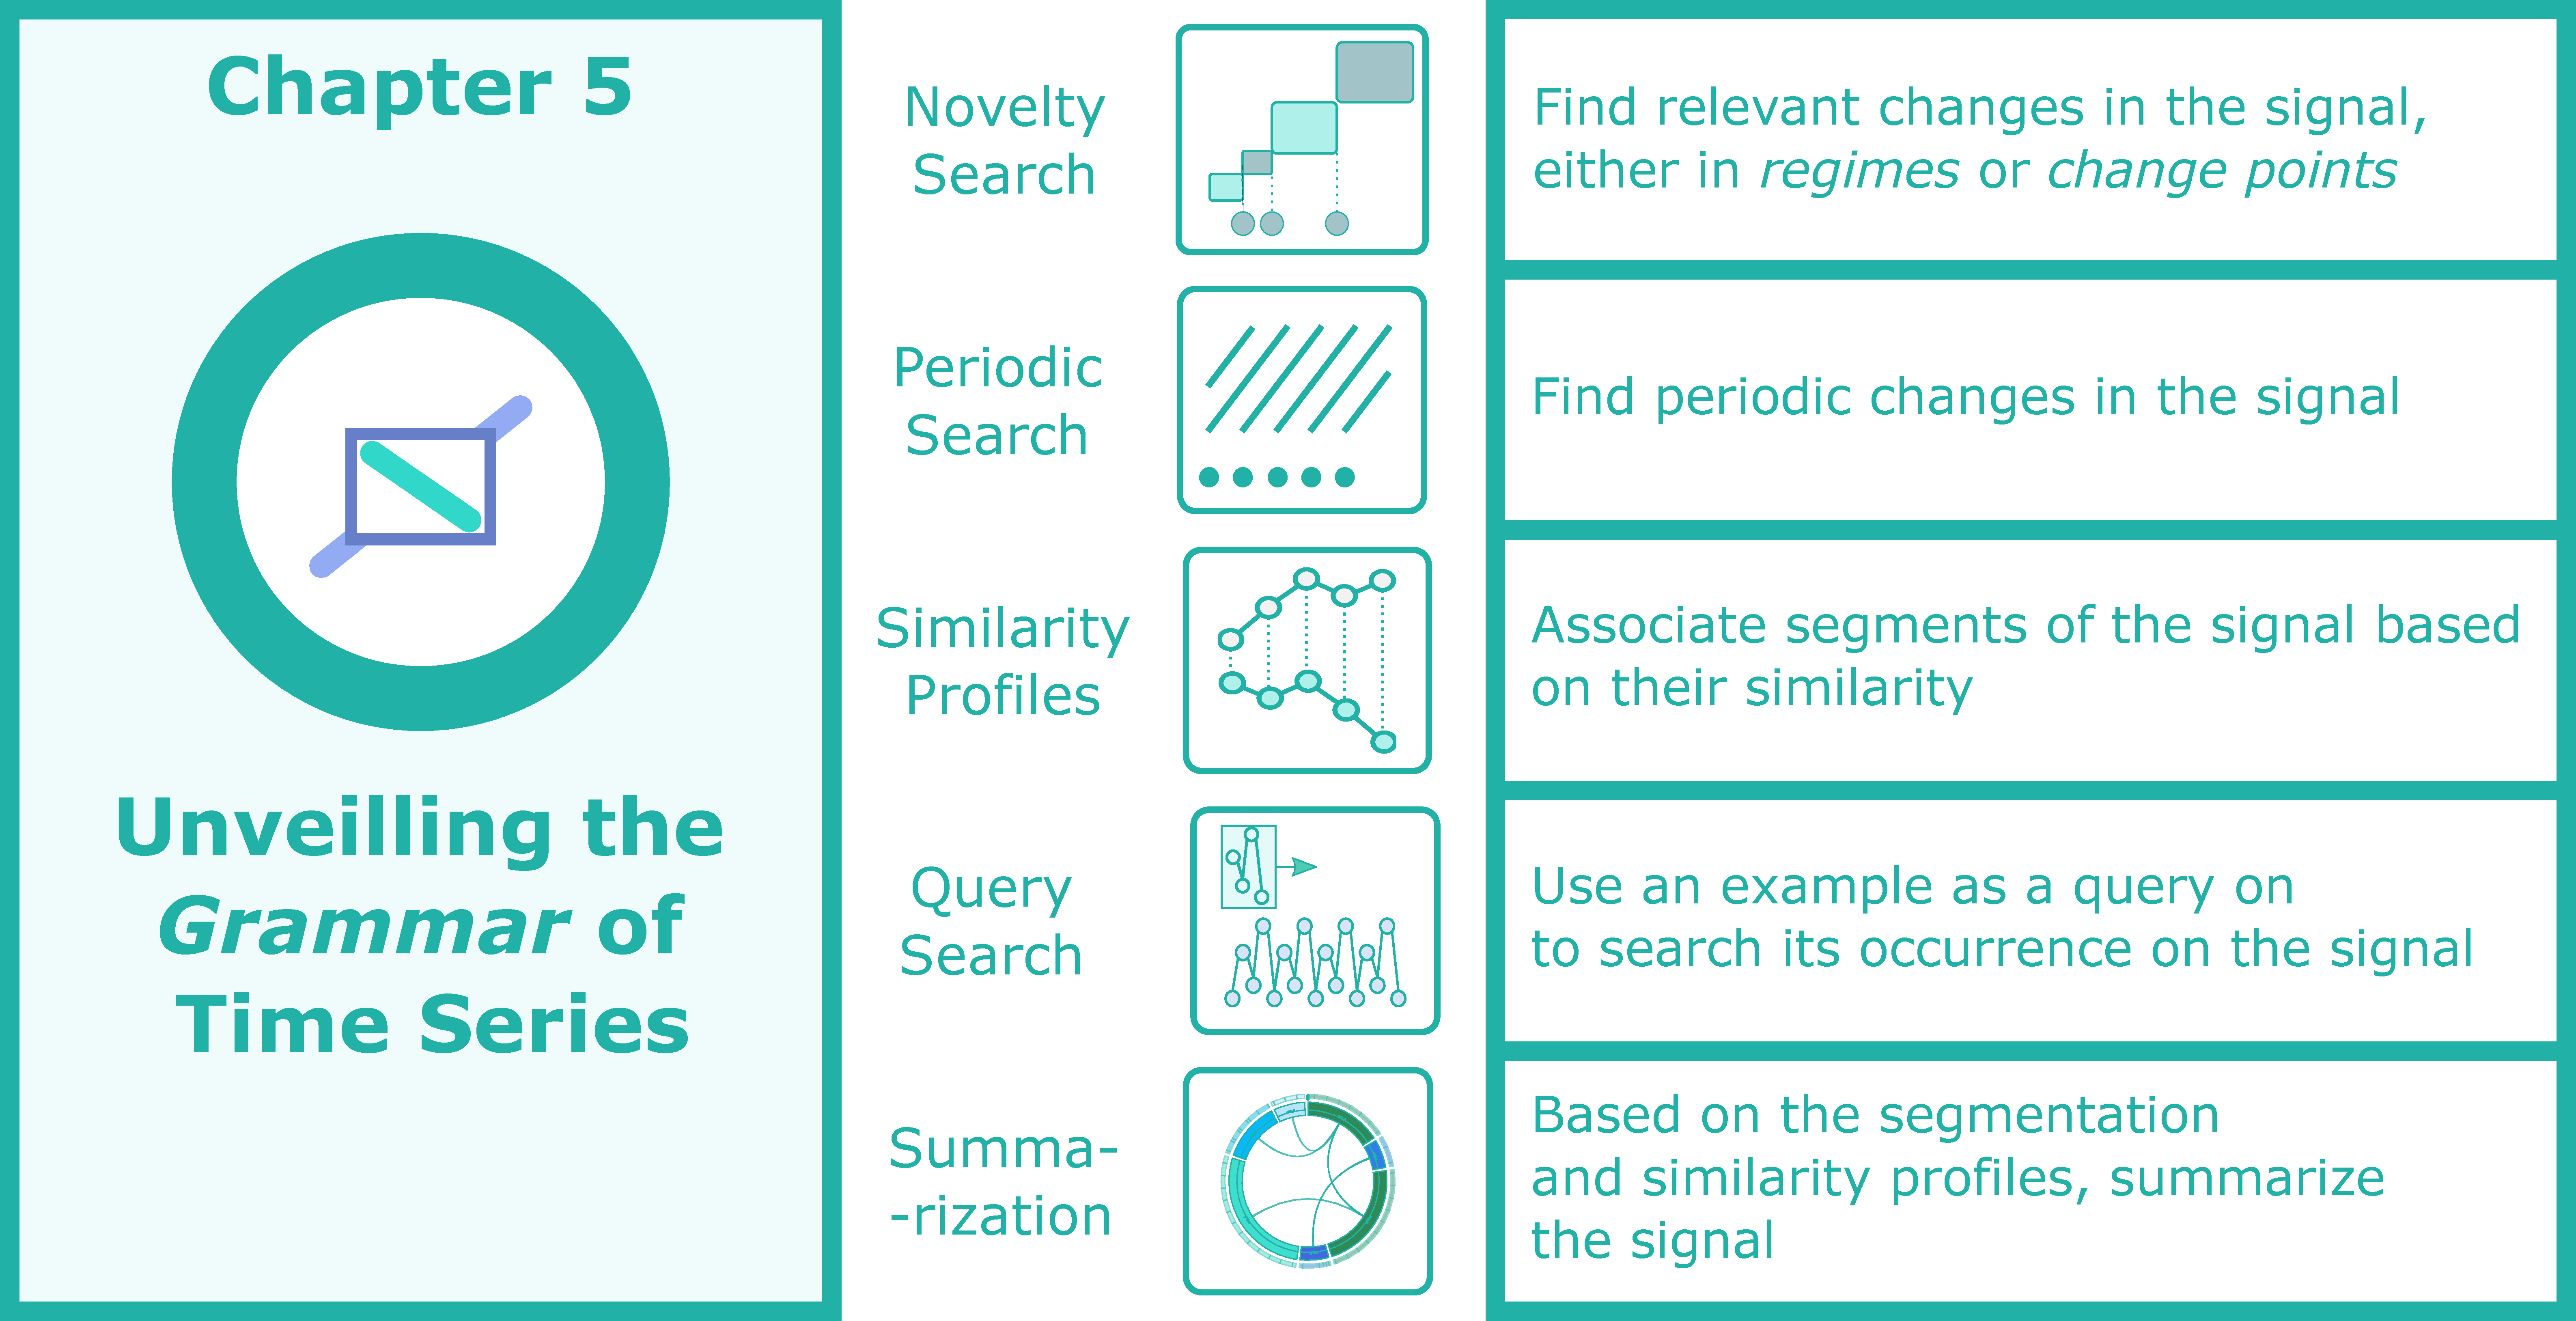
\includegraphics[width=\linewidth]{intro_chapter5.pdf}
\caption{Information retrieval topics explained in this Chapter. Each of these topics is a result of analysing the \gls{ssm}.}
\label{fig:info_retrieval_topics}
\end{figure}

Researchers are interested in understanding the structure of the recorded signals, the meaning behind them, and the influences of the context. In Chapter 1 (see Section \ref{sub:context1}) we gave several examples of how signals in our everyday life can be structured and partitioned, such as a signal representing a \textcolor{myblue}{walking} regime shifting to a \textcolor{mygreen}{jogging} regime (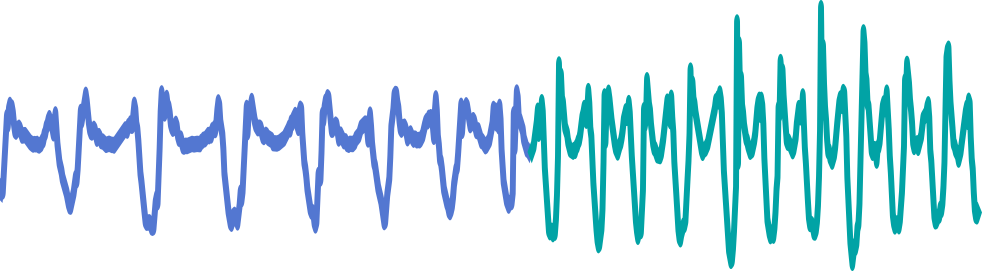
\includegraphics[height=5ex, valign=m]{walking_jogging.png}). The examples we mentioned in Chapter 1 and above manifest the relevance and importance of the following topics:

\begin{itemize}
     \item \textbf{Novelty segmentation}: to identify significant changes in the signal's behaviour.
    \item \textbf{Periodic segmentation}: to detect the presence of repeating cyclic patterns.
    \item \textbf{Labelling}: to measure how similar the segments are between each other with the help of similarity profiles.
    \item \textbf{Query search}: to find repeating patterns in the time series based on a \textit{subsequence} given as an example.
    \item \textbf{Summarization}: to summarize visually the time series by partitioning it into relevant and uniform/periodic segments and joining segments based on their similarity.
\end{itemize}

In this Chapter, we present the proposed solutions to the five problems mentioned above, which are inspired by a method used for audio signal analysis and thumbnail generation \cite{fmp1, audiolabs1, audiolabs2, cpd_audio}. Such a method has not yet been extended to other types of \textit{time series} domains that could greatly benefit from it \cite{muller_music_health}. The method uses a feature-based \gls{ssm} of (multidimensional) time series, from which visual and analytical information is rendered to perform the segmentation process and associate \textit{subsequences} of the time series with each other. This association based on similarity can be used towards automatic labelling and ultimately to summarize the signal. We extended its application to \textit{biosignals} with the usage of general features and introduced new methods to analyse the \gls{ssm} for periodic segmentation, labelling, query search, and summarization.


\section{The Problem}

Defining what is relevant in a time series highly depends on the context and purpose of the analysis, but globally, for any type of time series, there is a general interest in understanding how the signal is structured and how are \textit{subsequences} related, especially for tasks related to data labelling. The structure of a time series is built of \textit{segments} delimited by \textit{events}. The problem explored in this section is the search for such \textit{events} and how to find the ones that are significant and useful to then perform a similarity search and summarization of the time series.
\par
From the definition of \textit{event} (see Chapter 2 Section \ref{sec:global}), we highlight two primary considerations for the detection of events: (1) an event is a change in the behaviour of the time series, and (2) it has to be significant both \textit{statistically} and \textit{qualitatively}. The \textit{qualitative} aspect indicates subjectivity from the analyst because of the domain or context of the problem. Considering this, we will start by explaining the dimensions of the problem: (1) search and (2) type of significance. 

\subsection{Search Ranks}

\begin{figure}
    \centering
    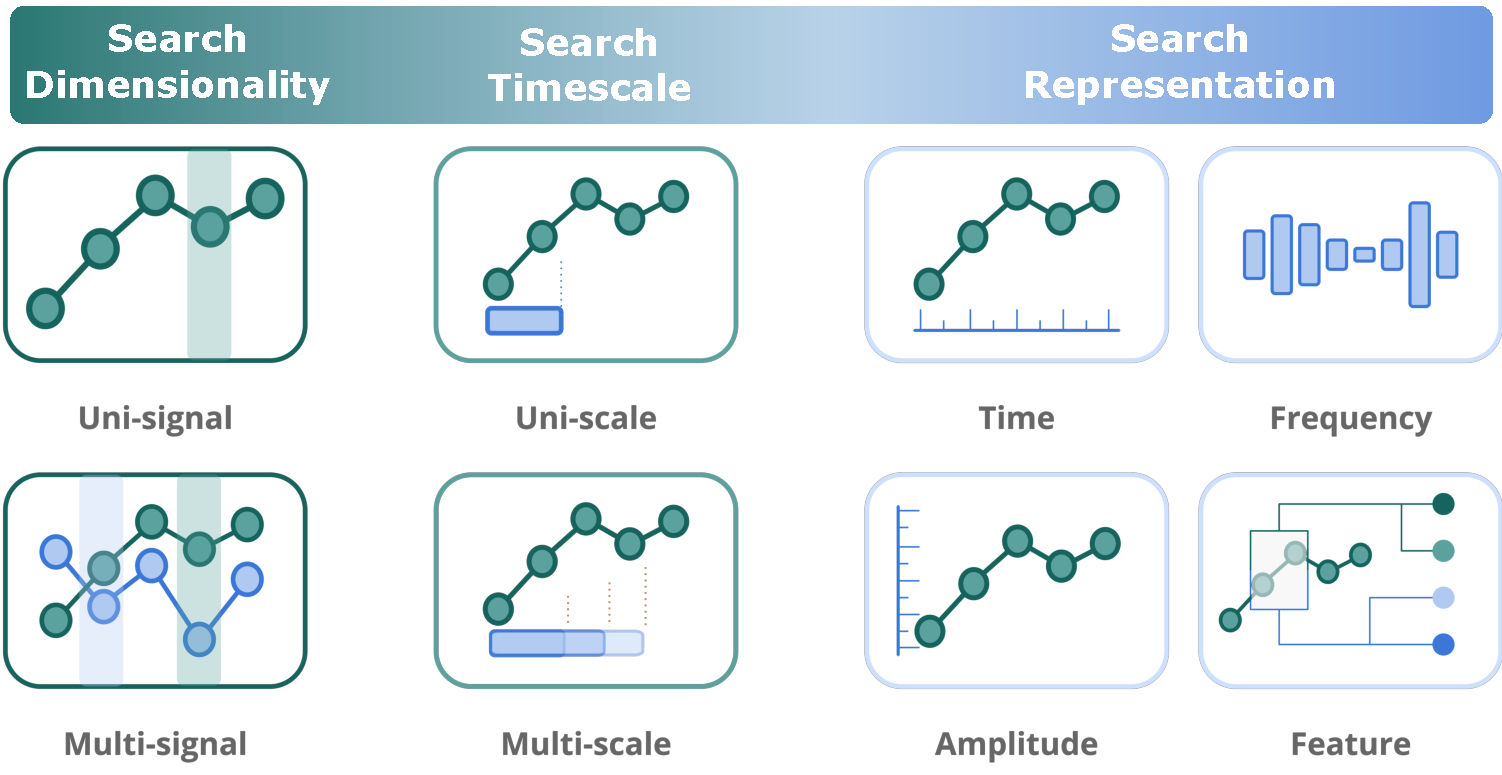
\includegraphics[width=0.8\linewidth]{event_search.pdf}
    \caption{Event search in different ranks of dimensionality, timescales, and representation.}
    \label{fig:event_search}
\end{figure}


%\begin{figure}
%\begin{subfigure}{.5\textwidth}
%	\centering
%	\includegraphics[width=0.95\linewidth]{event_search.png}
%	\label{fig:event_search}
%	\caption{}
%\end{subfigure}%
%\begin{subfigure}{.5\textwidth}
%	\centering
%	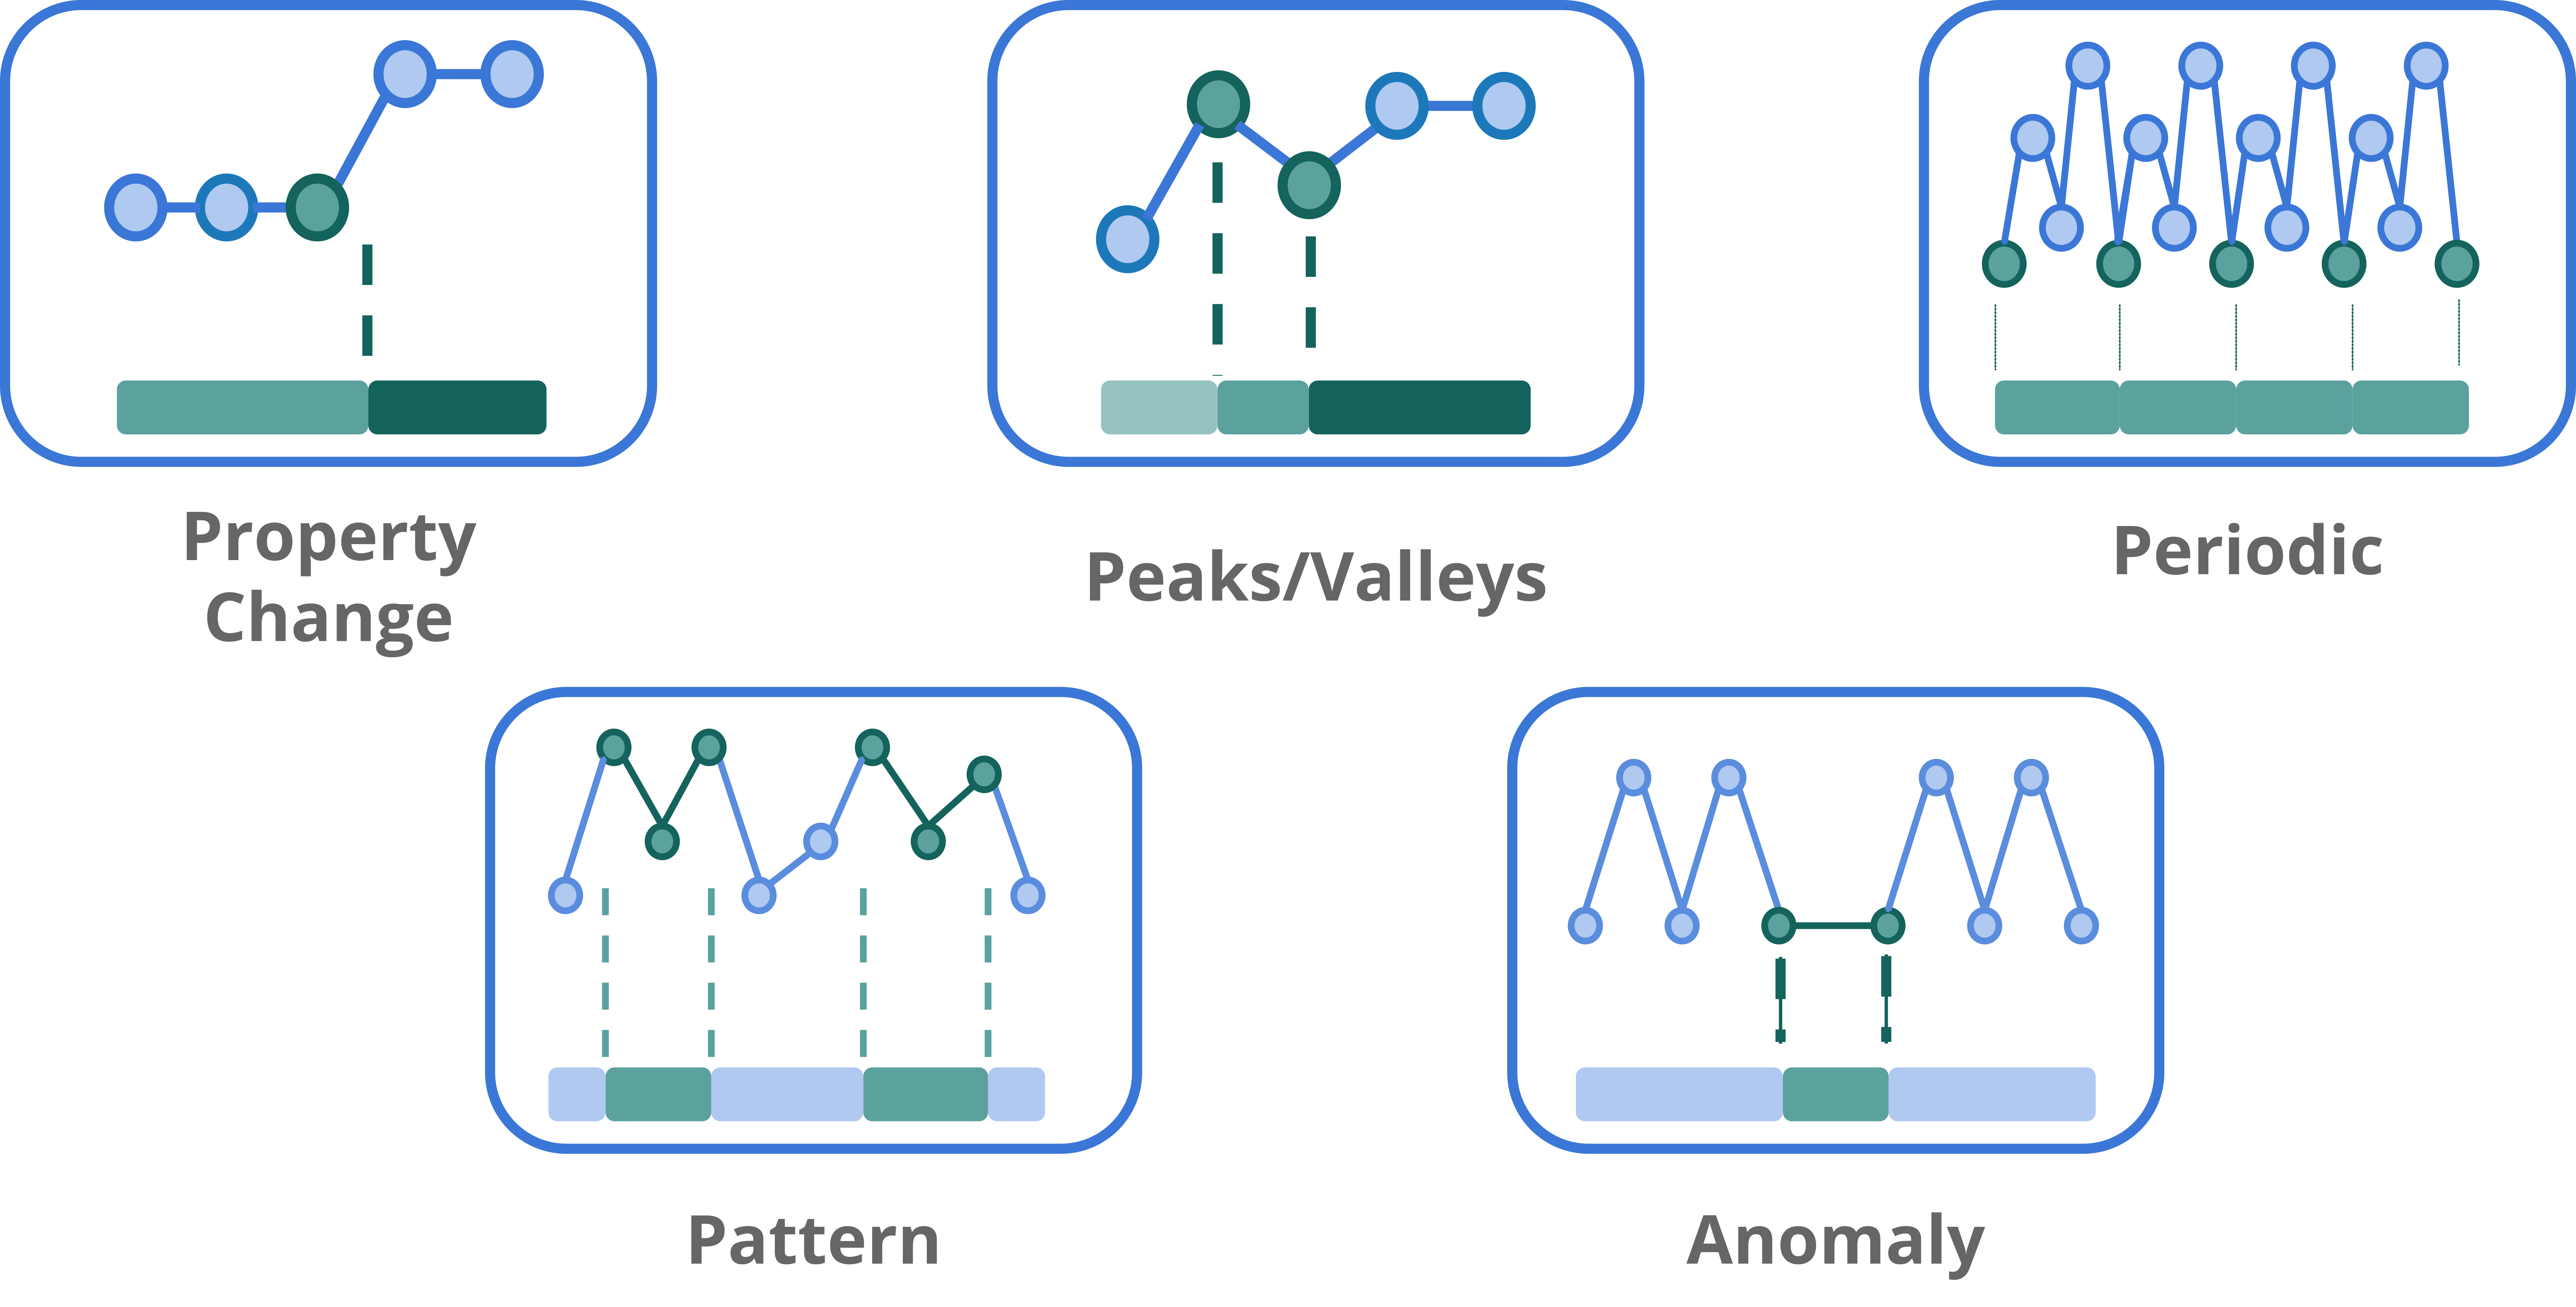
\includegraphics[width=0.95\linewidth]{event_type.png}
%	\label{fig:event_type}
%	\caption{}
%\end{subfigure}
%\caption{(a) Categories of search of events. In this case are shown Dimension, Window, and Domain. (b) Examples of different types of events that can be considered significant in a time series.}
%\end{figure}


Figure \ref{fig:event_search} illustrates the search ranks of the problem formed by three layers:

\begin{itemize}
    \item \textbf{Dimensionality}: The search can be applied to one or multiple time series. In multidimensional space, some events can coincide in several time series, while others are specified on a particular dimension. For example, some gestures produce noticeable signals on only one dimension of the three-axis accelerometer.
    \item \textbf{Timescale}: \textit{Events}' occurrence can vary from different timescales. For example, when the signal being analysed is zoomed in from hour to minute scales, some events may disappear while new events may be detected.
    \item \textbf{Representation}: The searchable objects can be straightforwardly the temporal nature of time series or other representation, such as frequency or other extracted features.
\end{itemize}

Besides the ranks mentioned above, the search procedure can be customized by context or target, which is highly related to the relevance given to an \textit{event} or a \textit{subsequence}. Types of events that are considered significant include:

\begin{itemize}
  \item \textbf{Property change}: The change of a property, such as a change in mean or frequency, or a set of properties is greater than a threshold, e.g., \textcolor{myblue}{low} to \textcolor{mygreen}{high} frequency - 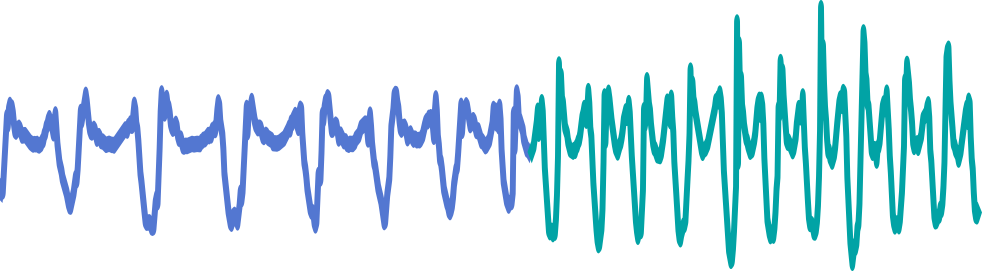
\includegraphics[height=2.5ex, valign=m]{walking_jogging.png}.
  \item \textbf{Peak/Valley}: Peaks and valleys can typically be associated with significant physical changes, e.g., \gls{ecg} \textcolor{mygreen2}{peaks} like 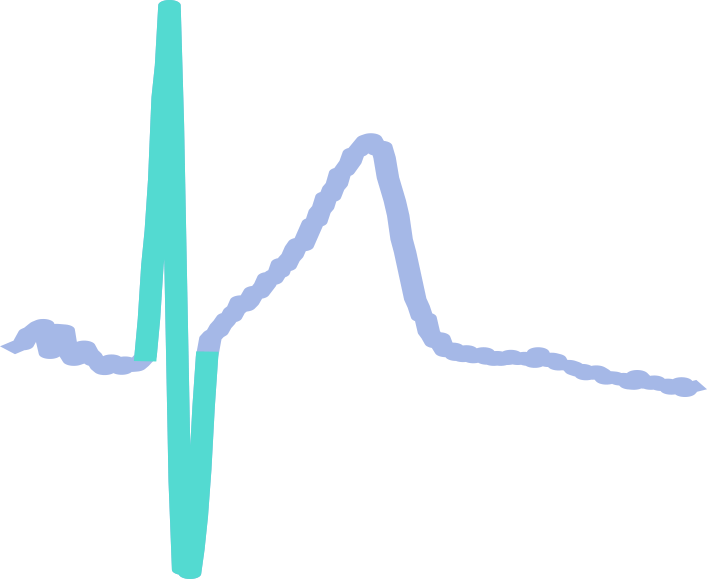
\includegraphics[height=3.5ex, valign=m]{high_peak_ecg.png}.
  \item \textbf{Periodicity}: The starting points of each period in a periodic signal are considered relevant, e.g., \gls{abp} periods like 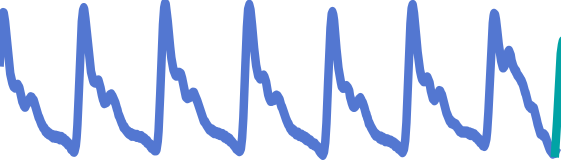
\includegraphics[height=2.5ex, valign=m]{bvp_segment.png}.
  \item \textbf{Recurrent pattern}: Re-occurrences of similar \textit{subsequences} with specific patterns should be of interest. Unlike \textit{periodicity}, \textit{recurrent} patterns do not have a temporal regularity, e.g., the \textcolor{myblue}{arrhythmias} found in an \gls{ecg} signal like 
\includegraphics[height=3ex, valign=m]{arrhytmia_thumbnail.pdf}.
  \item \textbf{Anomaly}: Highly dissimilar \textit{subsequences} with particular patterns are of the reference value, e.g., \textcolor{myred}{noise} in a clean signal 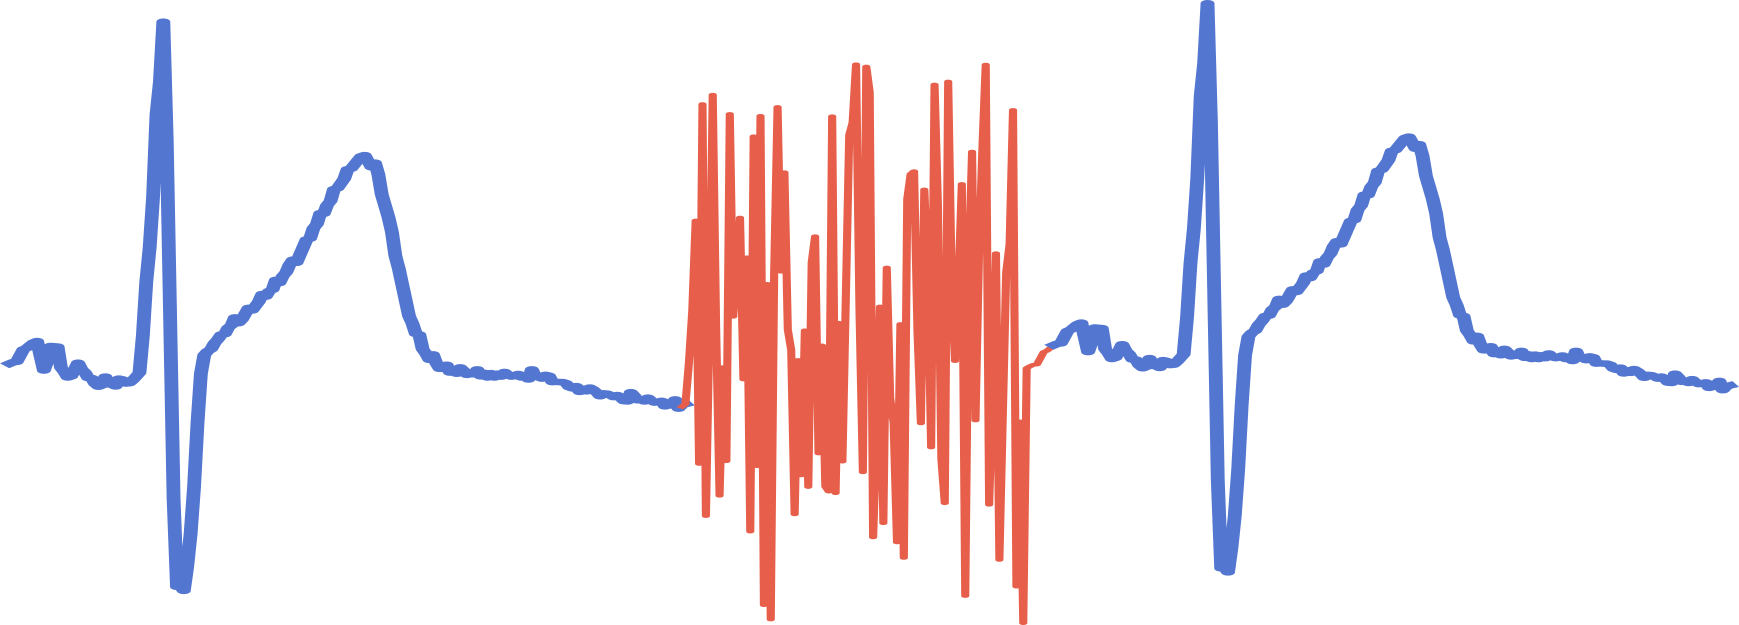
\includegraphics[height=3ex, valign=m]{ecg_noise_thumbnail.png}.
\end{itemize}

%Figures \ref{fig:event_search} and \ref{fig:event_type} are an illustrated summary of the two dimensions of the problem. Regarding the \textit{search} dimension, it is formed by three layers: \textit{(1) dimensionality}: the search can be made in one or multiple time series. In the multidimensional space, events can occur simultaneously in several time series, but other events can be specified for each of them (e.g. an accelerometer signal has 3 dimensions, but some gestures might be noticeable in only one of them); \textit{(2) time scale}: \textit{events} might occur in different time scales (e.g. when looking into a time series of 1 hour long, we might see some relevant events, but when looking for a \textit{subsequence} of 10 minutes (zooming-in), other events are revealed); \textit{(3) domain}: the search procedure might be made directly on the time series using time properties, a distance measure (e.g. \gls{ed}), or can be made on another representation level, such as the feature domain.
%
%In what regards the \textit{event} type, we show in Figure \ref{fig:event_type} examples of events that are considered significant in a time series: \textit{(1) Property change:} when the change of a property or set of properties is greater than a threshold, such as changes on the mean (FIND THUMBNAIL IMAGE) or frequency (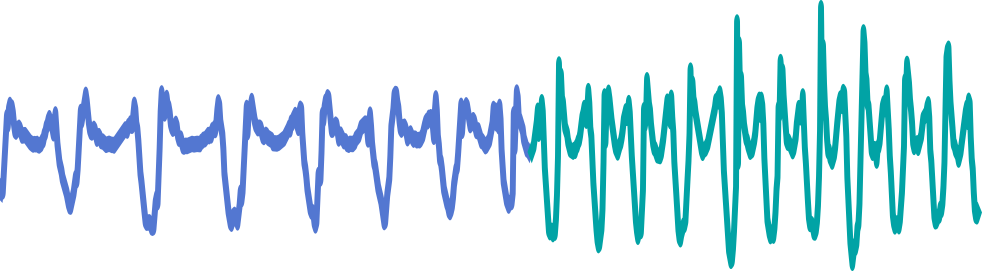
\includegraphics[height=3.5ex, valign=m]{walking_jogging.png}), \textit{(2) Peak/Valley}: peaks and valleys can typically be associated with significant physical changes (e.g. the peaks of an \gls{ecg} signal 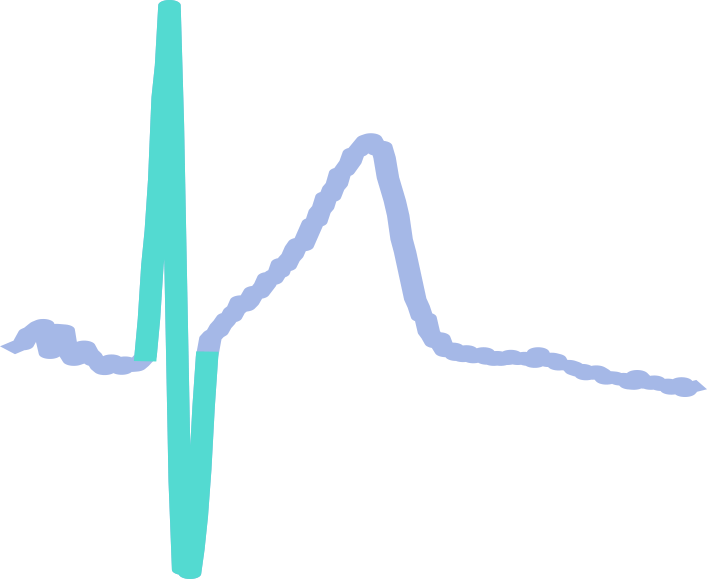
\includegraphics[height=3.5ex, valign=m]{high_peak_ecg.png}), \textit{(3) Periodicity}: if a signal is periodic, the moment each period starts is considered relevant (e.g. the cycles of a BVP signal 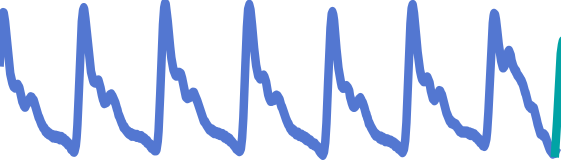
\includegraphics[height=2.5ex, valign=m]{bvp_segment.png}), \textit{(4) recurrent pattern}: re-occurrences of similar \textit{subsequences} with a certain shape or \textit{(5) anomaly}: very dissimilar \textit{subsequences} are relevant to indicate (e.g. noise in a clean signal 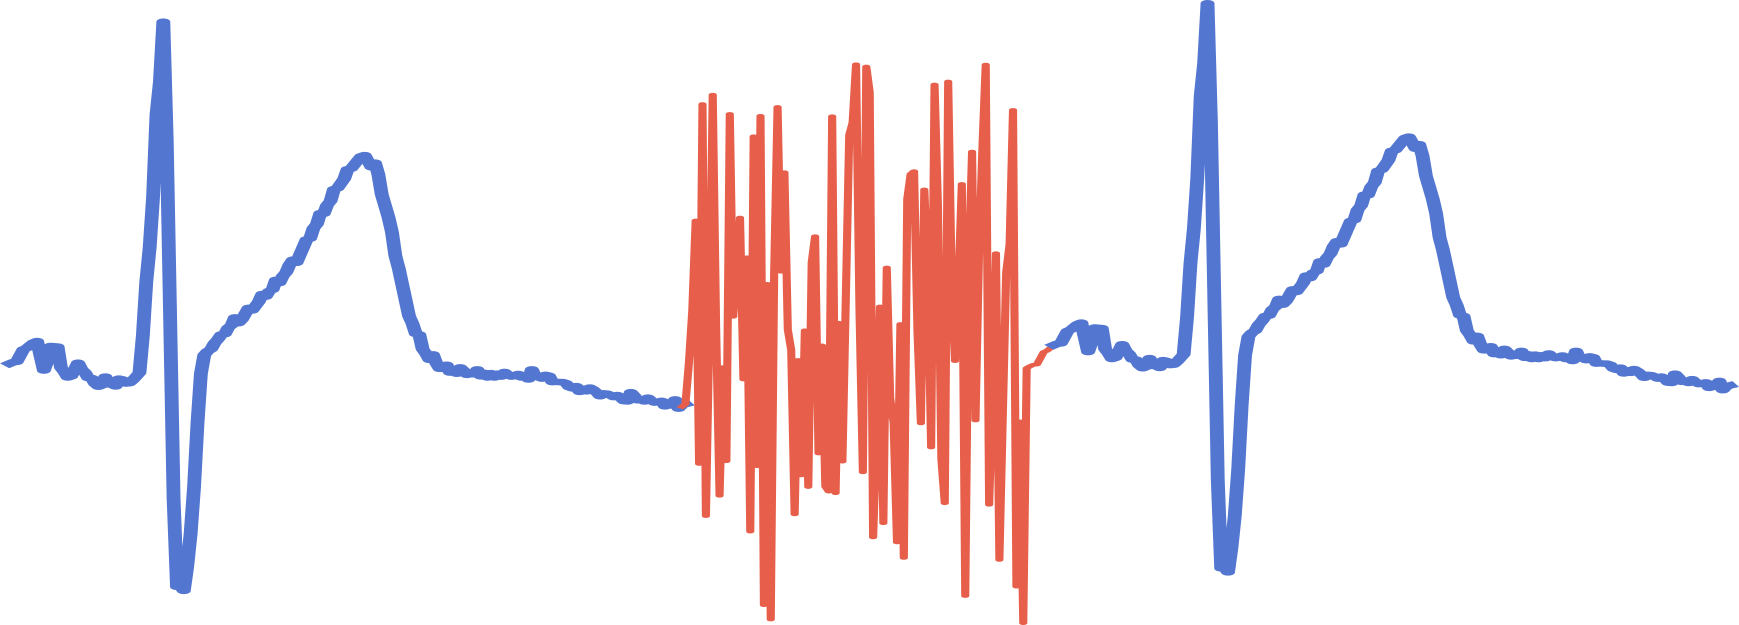
\includegraphics[height=3ex, valign=m]{ecg_noise_thumbnail.png}).

\subsection{Proposal}

In order to fill as many research gaps as possible, this study started by defining the search space for the aforementioned topics, considering that if the time series is transformed in the feature space, we can have a multidimensional similarity analysis based on the features' behaviour. The notion of \textit{difference} in time series can be associated with \textit{distance/similarity}, enabling finding segmentation points, recurrent patterns, anomalies, and periodic shapes, which is ideal to perform all the approaches listed above. This feature-based multidimensional representation is already successfully used for time series' classification purposes \cite{barandas_tsfel_2020} and is potentially applicable to all the mentioned topics. 
For instance, any feature's change would be relevant for novelty segmentation, such that changes in the mean, standard deviation, frequency, or other properties are all options worth searching for. By characterizing the signal in the feature space, we can explore changes in all feature representations.

We propose an unsupervised methodology that searches for events (1) in uni and multidimensional space, (2) with a fixed timescale and potential multi-timescale application opportunities, and (3) on an \gls{ssm} computed by a feature space representation of the time series. The events to be searched are any changes in the \gls{ssm} related to a segmentation point and/or a periodic event.
\par
The proposed method's reliability for event detection will be evidenced by considerable experiments in various type-agnostic databanks of multiple time series domains and comparisons to state-of-the-art methods. It should be highlighted that events in different datasets are extracted from the same information source, i.e., \gls{ssm}, which meanwhile provides insights into unsupervised automatic labelling.

    
%IMPORTANT
%Besides, at the feature level, we can very easily include the information of \textit{MTS}. The fact that features can be used for this purpose might help in targeting and fine-tuning the selection of features that work better for specific types of events or work domains (e.g. we might only be interested in changes related to the frequency and not mean fluctuations, therefore, frequency features should be chosen, making targeted event search).

%Tools: Annotation, Segmentation, One-click segmentation of periodic events, summarization, and profiling

\section{Building the Self-Similarity Matrix}

In this section, we explain the steps of the proposed method. The extraction of relevant events from time series starts by computing the \gls{ssm}. As explained in Section \ref{subsec:dist_matrix}, this matrix has relevant structural information to retrieve \textit{events}, namely \textit{blocks}, \textit{paths} and \textit{similarity profiles}. Figure \ref{fig:SSM_scheme} summarizes the steps involved in calculating the \gls{ssm}.

\begin{figure}
\centering
    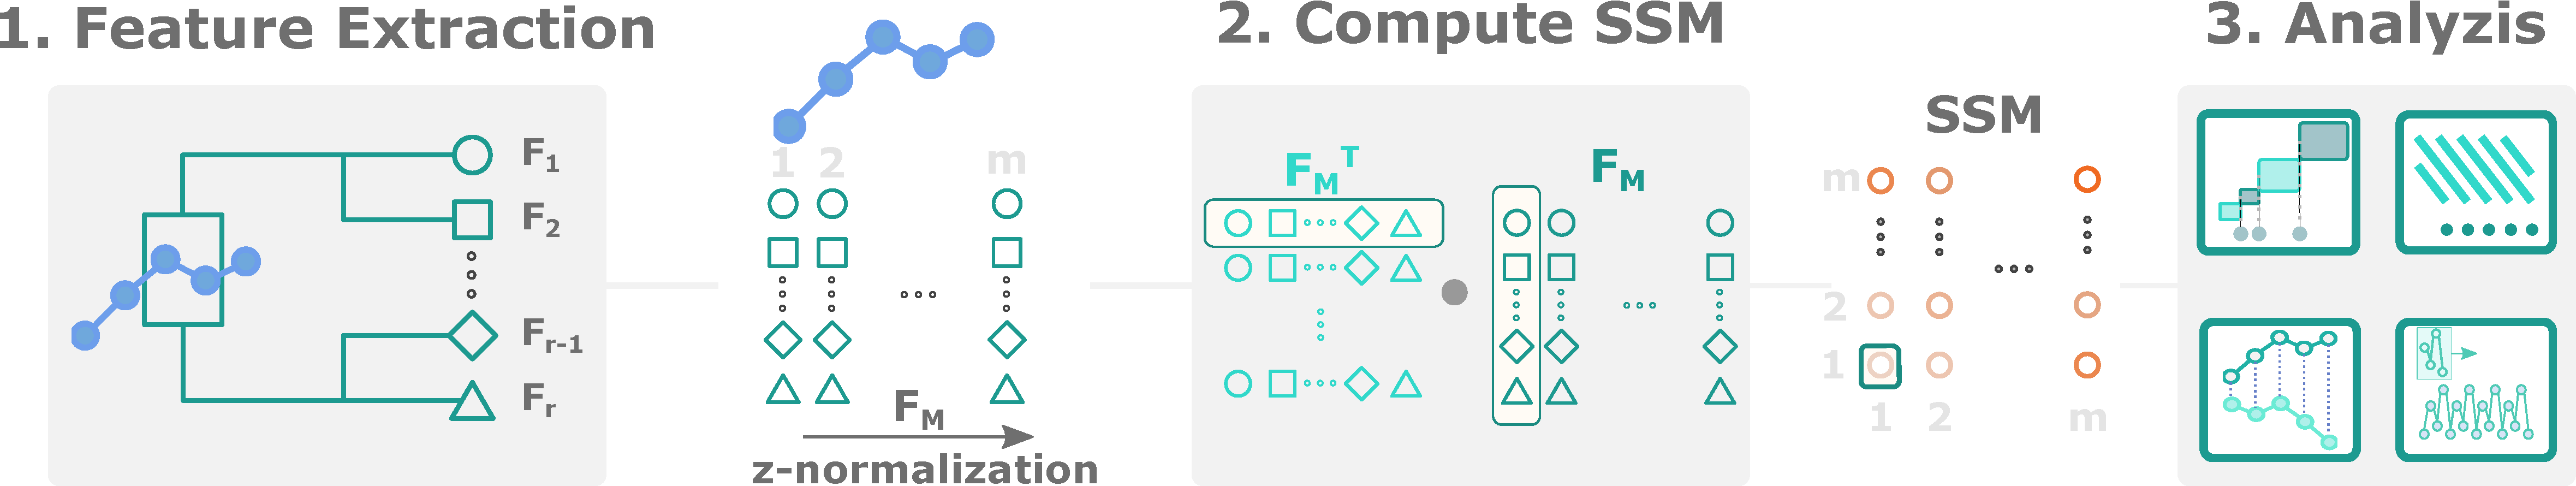
\includegraphics[width=\linewidth]{SSM_steps.pdf}
    \caption{A step-by-step flowchart for calculating and analysing the \gls{ssm}. The signal-based calculation requires input parameters of the window size $w$ and the overlapping percentage $o$ to fulfill the first-stage feature extraction. Features are extracted on each subsequence $(sT_1, sT_2..., sT_N)$, where $N$ is the total number of windows. $K$ features are extracted from window $i$ ($sT_i$: $f_{i_1}, f_{i_2}, ..., f_{i_K}$). Different features are associated with different shapes ($\bigcirc, \Box, \Diamond$, and $\triangle$) in the figures. The features can be extracted on an $M$-variable record and each feature is positioned as a row on the $F_M$ for the \gls{ssm} computation.}
    \label{fig:SSM_scheme}
\end{figure}

\subsection{Feature Extraction}

The structural information on the \gls{ssm} reflects how informative the feature set can translate the signal's changes and disruptions. Behavioural changes may be related to a variate set of features. As a feature can be sensitive to a particular type of change, the set of features should be diverse to identify a multivariate set of events and be agnostic to various signal types. We turned to the available features from the \textit{Time Series Feature Extraction Library} (TSFEL) \cite{barandas_tsfel_2020} for Python, which has been proven effective and efficient in our previous work on \gls{har} and multimodal biosignal processing \cite{liu22pipeline, liu2021thesis}. We selected over 50\% of all TSFEL features in the statistical, temporal, and frequency domains with relatively lower computational costs, as listed in Table \ref{tab:tsfel_featurelist} in Appendix \ref{app:tsfel}, regarding our proposed method's high calculation resource consumption.

The features are extracted with a moving window with size $w$, specified by the user, with an overlap percentage $o$. The selection of the two sizes significantly influences the results: $w$ defines the timescale at which features are extracted so that the wider the window, the more \textit{zoomed-out} the search will be. The second parameter defines the pixel resolution of the resulting feature series, increasing the amount of information with a larger overlap.

The extracted features are grouped into a feature matrix ($F_{M}$), where the rows represent a feature series and the columns correspond to all subsequences. In the multidimensional case, $r$ features extracted from each of the $k$ dimensions are ordered in the $F_M$ as rows, forming $r \times k$ elements in each row, as illustrated in Figure \ref{fig:SSM_scheme}.

\begin{figure}
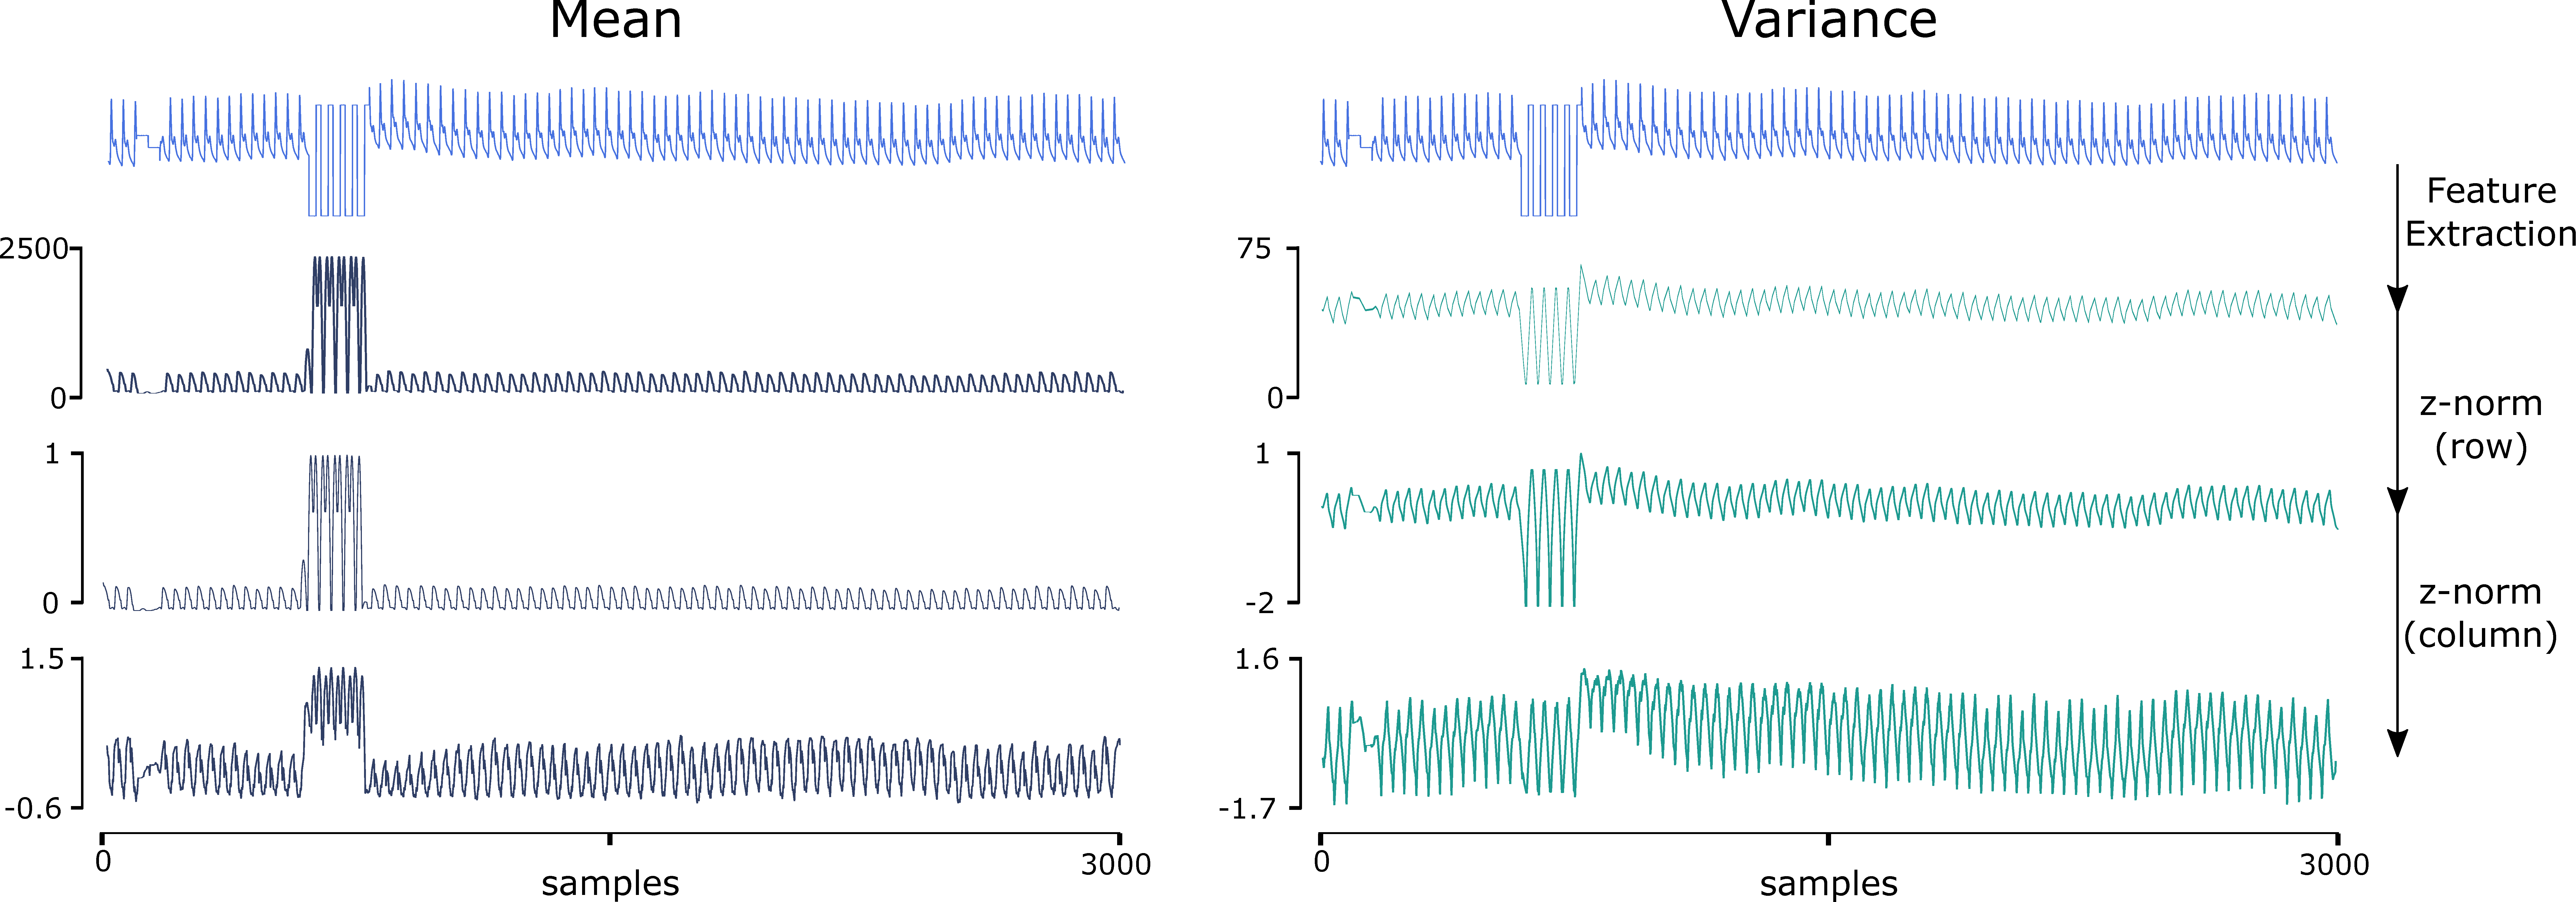
\includegraphics[width=\linewidth]{features_example.pdf}
\caption{Example of feature vectors before and after normalization. Mean and Variance features are presented for the \gls{abp} signal from Dataset \ref{dat:dataset2}.}
\label{fig:features_normalized}
\end{figure}

Each feature series (rows of the $F_M$) is z-normalized for a more balanced contribution to characterizing the signal. A further normalization is applied to the feature vector (columns of the $F_M$), which optimizes the cosine similarity computation between feature vectors by simply adding the dot product to calculate the \gls{ssm}. As an example of two simple features (mean and variance) and their normalized versions, we show Figure \ref{fig:features_normalized}.

\subsection{Feature-based SSM}
\label{sec:the_ssm}

After grouping all the features extracted, the next stage is to apply a similarity measure to the feature space and compute the \gls{ssm}. This process consists in comparing each \textit{subsequence} with all the other \textit{subsequences}. Since each column of the $F_M$ is each subsequence's feature characterization in the entire feature set, the \gls{ssm}, i.e., the comparison between segments, is obtained by calculating the dot product between the z-normalized transposed $F_{M}$ and itself:

\begin{equation}
    \SSM = F^T_M \cdot F_M.
\end{equation}

The dot product scores the similarity based on the subsequence's feature values. Cells of the \gls{ssm} with higher similarity scores indicate that the corresponding \textit{subsequences} have similar feature values \cite{audiolabs1, audiolabs2}. As a result, the \gls{ssm} provides rich visual information, highlighting structures that describe the signal's morphological behaviour over time and structure, such as blocks and paths.

\begin{figure}
    \centering
    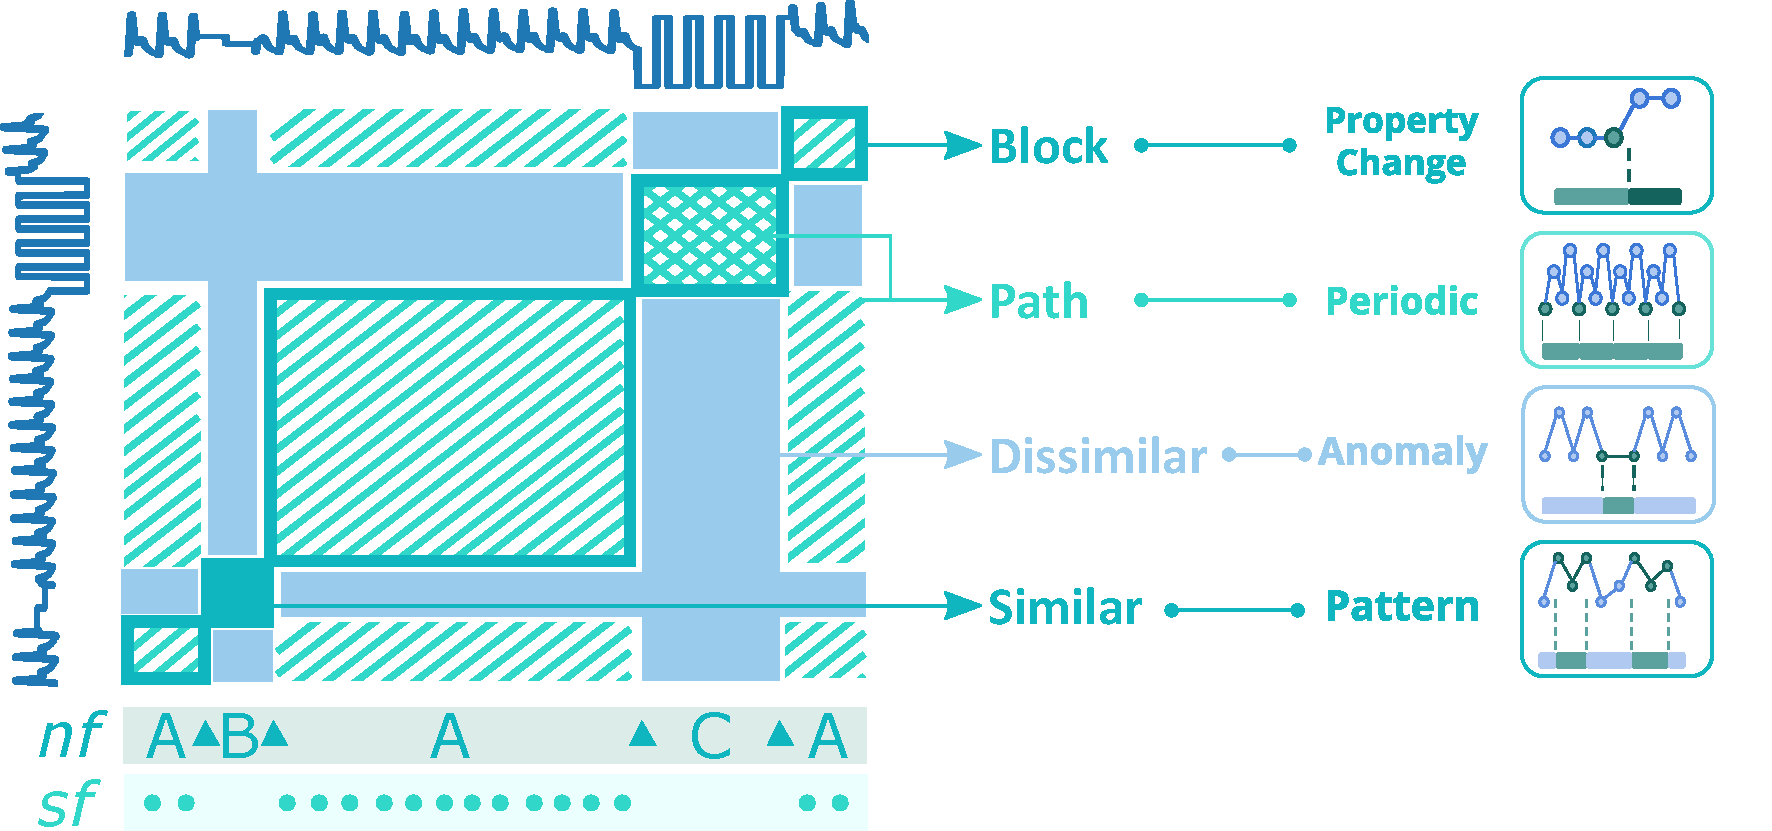
\includegraphics[width=\linewidth]{SSM_example.pdf}
    \caption{The informative structures of an \gls{abp} signal's \gls{ssm}. The three main structures are highlighted in the simplified illustration: A - the homogeneous segments corresponding to periods in the \gls{abp} signal; B - the homogeneous segment representing missing data; C - the homogeneous segment cueing sensor detachment. The ``blocks'' in the figure accentuate homogeneous behaviour while the paths in the figure depicts periodicity in the segment. Segment C has a cross pattern, which symbolizes periodicity and symmetry. $nf$: \textit{novelty function}; $sf$: \textit{similarity function}; $\triangle$: change points separating blocks A, B and C.}. 
    \label{fig:ssm_description}
\end{figure}

In Figure \ref{fig:ssm_description}, the main structures are illustrated and highlighted in an example of an \textit{\gls{ssm}} \cite{audiolabs1} computed from an \gls{abp} signal, where the main structures are \textit{blocks} and \textit{paths}. Our proposed method utilizes the resulting main structures to extract the desired information.
\textit{Paths} show recurrence of patterns, which indicates the morphological matching between corresponding \textit{subsequences}. Circles in the \textit{sf} layer exhibit when the paths start. The \textit{cross-pattern} in \textit{block} C means that the \textit{subsequences} are periodic and symmetric.

Differently, \textit{blocks} are square-shaped structures of homogeneous areas in the \gls{ssm}, translated as constant behaviour in the time series. The change between block structures along the main diagonal displays a relevant change in morphology and behaviour in the time series. In Figure \ref{fig:ssm_description}, the \gls{ssm} is segmented into several blocks on layer \textit{nf}, for which the $\triangle$s mark the change points that separate blocks A, B and C. Besides \textit{paths} and \textit{blocks}, the \gls{ssm} provides similarity measures between \textit{subsequences}, which can be used to spotlight (dis)similar segments, such as anomalies, motifs or cycles. Several strategies were applied to the \gls{ssm} to extract the mentioned information.

\section{Information Retrieval}

The \gls{ssm} is a powerful visual tool \textit{per se}, exposing relevant information that a raw observation could miss. Automatic discovery of information of interest will increase the \gls{ssm}'s practicability and versatility, for which three approaches for information retrieval on the \gls{ssm} are put forward: (1) novelty search of \textit{block} transitions, (2) periodic pattern search of \textit{paths}, (3) similarity profiles of \textit{subsequences}, and (4) how to use a query from the \gls{ssm} to search for specific \textit{subsequences}. 


\subsection{Novelty Search}
\label{sec:novelty_search}

The search for \textit{novelty} is inspired by a method used in musical structure analysis \cite{foote2000}, which is computed with the help of the \textit{libfmp} \textit{Python} package \cite{libfmp}. The process involves searching for transitions between \textit{blocks} using a moving chequerboard square matrix, resulting in a one-dimensional function: the \textit{novelty function}.


\begin{figure}
    \centering
    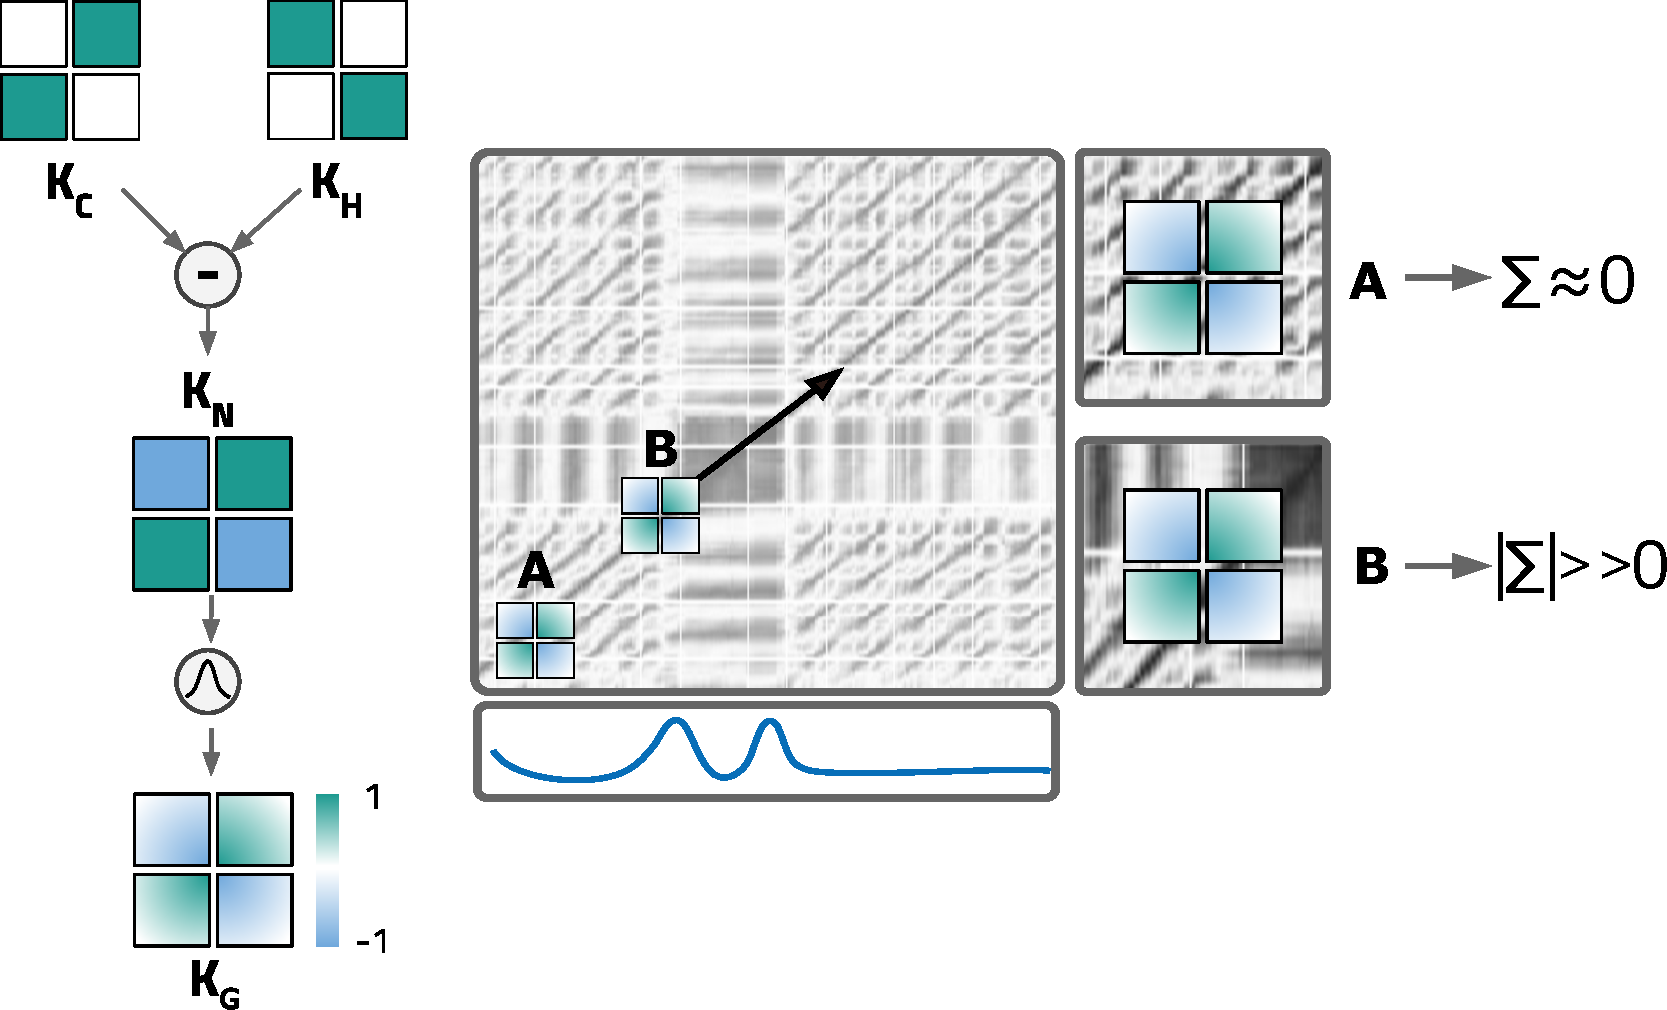
\includegraphics[width=\linewidth]{sliding_kernel.pdf}
    \caption{Left: description of the matrix (kernel) used to compute the \textit{novelty function}, based on the works of \textit{Mueller} \textit{et al.} \cite{fmp1, fmp2}. The chequerboard pattern of the kernel $K_N$ is achieved by combining the kernel $K_H$ (homogeneity measure) and $K_C$ (cross-similarity measure). Combined with a Gaussian function, the $K_G$ is obtained; right: the process to compute the novelty function based on the works of \cite{Dannenberg2008,fmp1, fmp2}. Kernel $K_G$ slides along the diagonal of the \gls{ssm} to compute the \textit{novelty function} presented as the bottom sub-plot. Positions A and B point to the effect of block transitions on the \textit{novelty function}.}
    \label{fig:kernel_description}
\end{figure}


As shown in Figure \ref{fig:kernel_description}, \textit{block} transitions along the diagonal are represented by a chequerboard pattern. Such patterns can be detected by correlating a standard chequerboard matrix with the diagonal of the \gls{ssm}, for which a sliding squared matrix, designated \textit{kernel}, is used. The kernel incorporates a Gaussian function with a smoothing factor. The kernel $K_N$ combines two different square matrices: $K_H$ and $K_C$. $K_H$ is responsible for identifying the homogeneity of the \gls{ssm} on each side of the centre – the more homogeneous the pattern is, the higher the corresponding values will be. $K_C$ measures the cross-similarity level. Therefore, when sliding the kernel $K_N$ along the diagonal, a higher correlation value will be returned when it reaches a segment of the \gls{ssm} with a similar chequerboard pattern. The result is the mentioned novelty function \cite{Dannenberg2008, fmp1, fmp2}.

In position \textbf{A} of Figure \ref{fig:kernel_description}(right), due to the high homogeneity, the kernel returns a value approaching 0 when summing the product between it and the section of the \gls{ssm} it overlaps. In contrast, the kernel in position \textbf{B} reaches a segment with low cross-similarity and high diagonal similarity, which results in high correlation values with a chequerboard pattern. Therefore, high \textit{novelty function} values are witnessed in these transition segments \cite{Dannenberg2008, fmp1, fmp2}.

Each section of the kernel has the same size, $L \in \mathbb{N}$, and $D = 2 \times L + 1$  configures the total kernel size. The kernel has an odd size to adapt zero values in centred points, and a total size of $D\times D$. $K_{N}$ is defined by \cite{fmp1, fmp2}:

\begin{equation}
        K_N(i,j)  = sign(a_i) \cdot sign(b_j),
\end{equation}

where $a,b\in[-L:L]$ and $sign$ represents the sign function (1, 0 or -1). A radially symmetric Gaussian function is used to smooth the Kernel \cite{fmp1, fmp2}:

\begin{equation}
    \phi(p,u) = \exp(-\frac{1}{2L\sigma^2}(p^2 + u^2)),
\end{equation}

where $\sigma$ is the standard deviation, equal for both $x$ and $y$ dimensions of the matrix, $L$ the size of each kernel's section, and $p$ and $u$ the position in the $x$ and $y$ dimensions, respectively. The kernel $K_G$ is computed by point-wise multiplication with the Gaussian function:

\begin{equation}
    K_{G} = \phi \cdot K_{N}    
\end{equation}

The \textit{novelty function} $n_f$ is calculated by correlating the kernel with the diagonal of the matrix:

\begin{equation}
    n_f(m) = \sum^{2L+1}_{i,j=0} K_{G}(a_i,b_j)\SSM(m+a_i, m+b_j)
\end{equation}

being the sample of the novelty function $m \in [0-N]$ and $a, b \in [-L:L]$. The change point events are represented by local maxima (peaks) in the \textit{novelty function}, which can be detected by standard peak-finding strategies.

\subsection{Periodic Search}
\label{sec:periodic_search}

As aforementioned, \textit{paths} indicate the presence of similarity and reoccurring patterns can be visualized on the \gls{ssm}. The \textit{path}'s start point punches where the period of the pattern begins. In order to find the periodicity, we compute the similarity function $s_f$ by summing the values of the symmetric \gls{ssm} column-wise or, equally, row-wise. Each element of the $sf$ is calculated by

\begin{equation}
sf(x) = \sum_{i=0}^{m}{\SSM_{ix}},
\end{equation}

\noindent where \textit{i} is the column position for the sum, $sf_{j}$ is the sample of the function at position \textit{j} and \textit{m} is the feature-series size. As segments with similar morphology will be closely described by the extracted features, the columns will have an approximate representation, resulting in similar values on the \textit{sf}. The similarity function will enhance such behaviour when facing periodic series. The identification of events related to the periodicity of a time series is then feasible by searching for local minima (valleys) on the similarity function.

Although not validated in this work, an additional application of the similarity function should be outlooked. Considering that each sample of the $sf$ is an average similarity of a subsequence to all other subsequences, it is possible to find \textit{anomalies}. Regarding an \textit{anomaly} as a subsequence highly unique and different from all the rest of the time series, its average similarity to all the other subsequences should have a low value.

\subsection{Similarity Profiles}
\label{sec:similarity_profiles}

The principal elements, \textit{blocks} and \textit{paths}, are the information basis for segmenting the time series. Besides, \gls{ssm} also provides pairwise similarity values between all \textit{subsequences} of the time series, an important measure that can be used for clustering and \textit{motifs}/\textit{discords} discovery. The similarity profiles exploit the similarity values of the \gls{ssm} to facilitate \textit{subsequences} comparison. 
A similarity profile charts the similarity values of a \textit{subsequence} (one column/row of the \gls{ssm}) to all the other \textit{subsequences}. The higher the values, the more similar the \textit{subsequences}. In addition to the \textit{subsequences} comparison, the similarity profile can also compare between entire segments of the signal. Consider, for instance, all three $A$-segments highlighted in Figure \ref{fig:ssm_description}, whose profiles are highly similar despite the different sizes. 

Although the segment comparison could be directly based on the region of the \gls{ssm} delimited by two \textit{subsequences}, we propose a more effective measure of two segments' similarity/difference according to their similarities/differences to all the other \textit{subsequences}. A \textit{similarity profile} $P_s(c)$ of a segment is computed as the column(row)-wise average similarity values of the region delimited by the segment being profiled (size $l$), and all the other \textit{subsequences} of the time series (size $m$):

\begin{equation}
P_s(c) = \frac{\Sigma_{i=0}^l SSM(i, c)}{l}.
\end{equation}

The \textit{similarity profile} is computed column(row)-wise. Each column(row) $c(r)$ is the average similarity value between the reference segment and the segment corresponding to $c$. The reasoning is that similar segments should have closer \textit{similarity profiles}. Since the profiles have the same size, they can be compared by certain distance measures, such as the \gls{ed}, to form clusters, an automatic clustering solution based on the segments generated by the \textit{novelty} and \textit{similarity} functions.

\begin{figure}
\centering
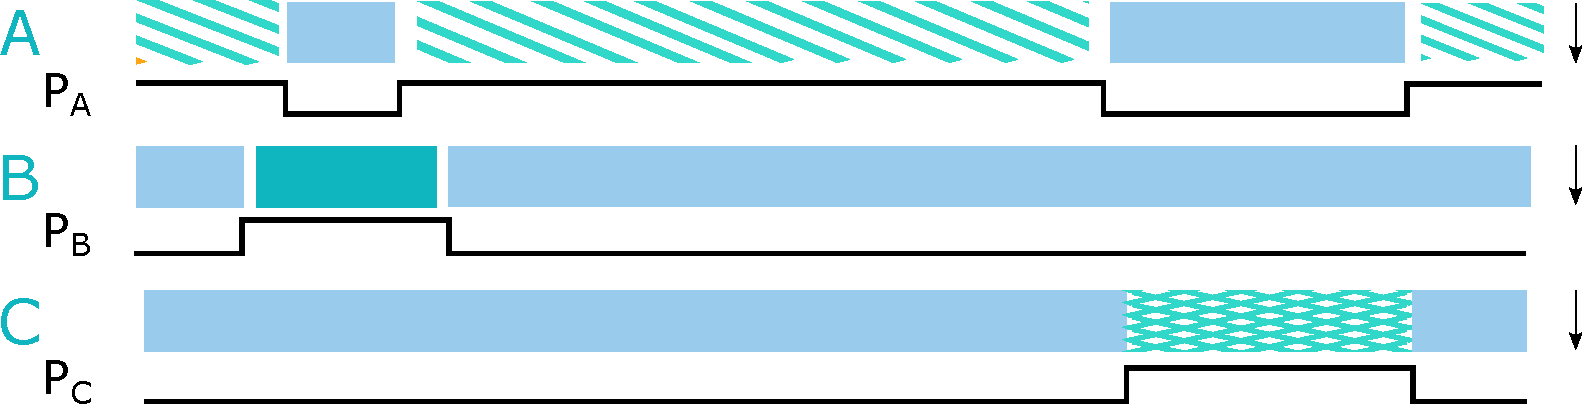
\includegraphics[width=\linewidth]{profiles.pdf}
\caption{Profiles computed for each segment of the example signal used in Figure \ref{fig:ssm_description}.}
\label{fig:profiles}
\end{figure}

A general example of applying this process to the segmented time series based on the \textit{novelty function} is shown in Figure \ref{fig:profiles}. Each segment category ($A$, $B$ and $C$) extracted from the \gls{ssm} of Figure \ref{fig:ssm_description} is computed into a profile ($P_A$, $P_B$ and $P_C$) by averaging column-wise. These \textit{similarity profiles} show how similar the segment is with all the other \textit{subsequences} of the time series. All segments $A$ will have a similar $P_A$ while being very different from profiles $P_B$ and $P_C$. 

\subsection{Query Search}
\label{subsec:query_based}

The mentioned similarity profiles are also useful to search for specific repetitions of a query from the time series. The process follows the traditional methods of template-based search methods explained in Chapter \ref{subsec:query_based_search}, but instead of doing the process directly on the time series, it is performed on the \gls{ssm}. The search procedure works by sliding the smaller column window (the example selected on the time series) along the \gls{ssm}, one sample at a time. The distance, $D$, between the example and the segment it slides over is calculated through the sum of absolute differences:

\begin{equation}
\label{eq:subsec_search}
    D(i) = \sum_{i=0}^{i=m}{\sqrt{(\SSM(i) - \SSM_t)^2}},
\end{equation}

where $\SSM(i)$ is the segment of the \gls{ssm} over which the example, $\SSM_t$, slides at moment $i$, up to the size of the \gls{ssm}. The resulting distance function has minimums at the position where the example is matched.

\section{Illustrative Evaluation in Various Application Scenarios}
\label{sec:use_cases_ssm}


Experiments from multiple domains were carried on to validate the practicability and universality of the process to represent the time series into a feature-based \gls{ssm} and the methods of retrieving information from the \gls{ssm}.

\subsection{Acceleration Signals in Human Activity Domain}
\label{sec:acc_har}

\begin{figure}
    \centering
    \begin{subfigure}[b]{\textwidth}
        \centering
        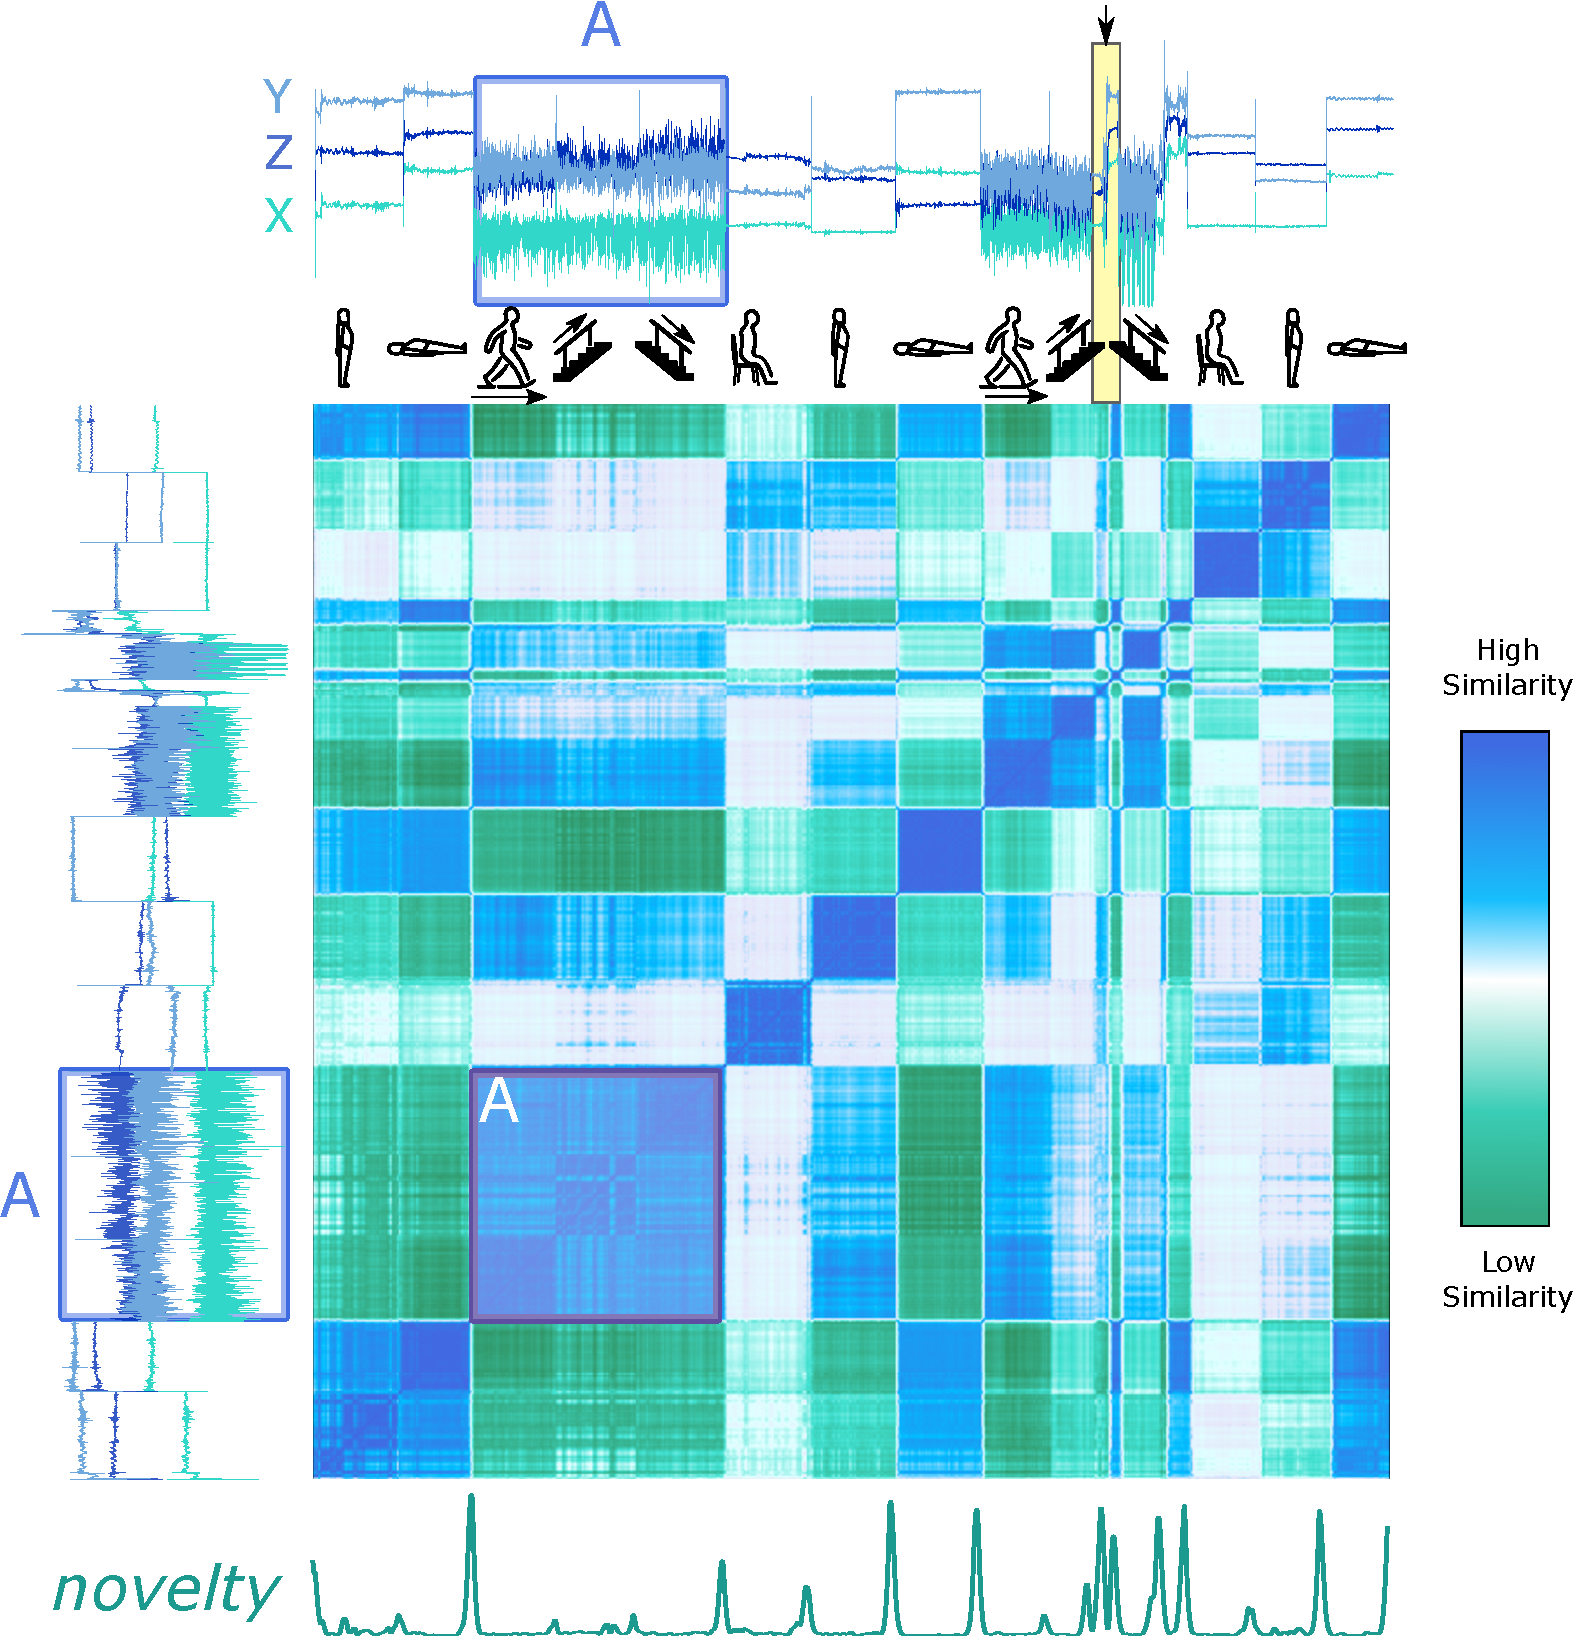
\includegraphics[width=0.8\textwidth]{use_case1_HAR.pdf}
    \end{subfigure}\\
    \vspace{2mm}
    \begin{subfigure}[b]{\textwidth}
         \centering
        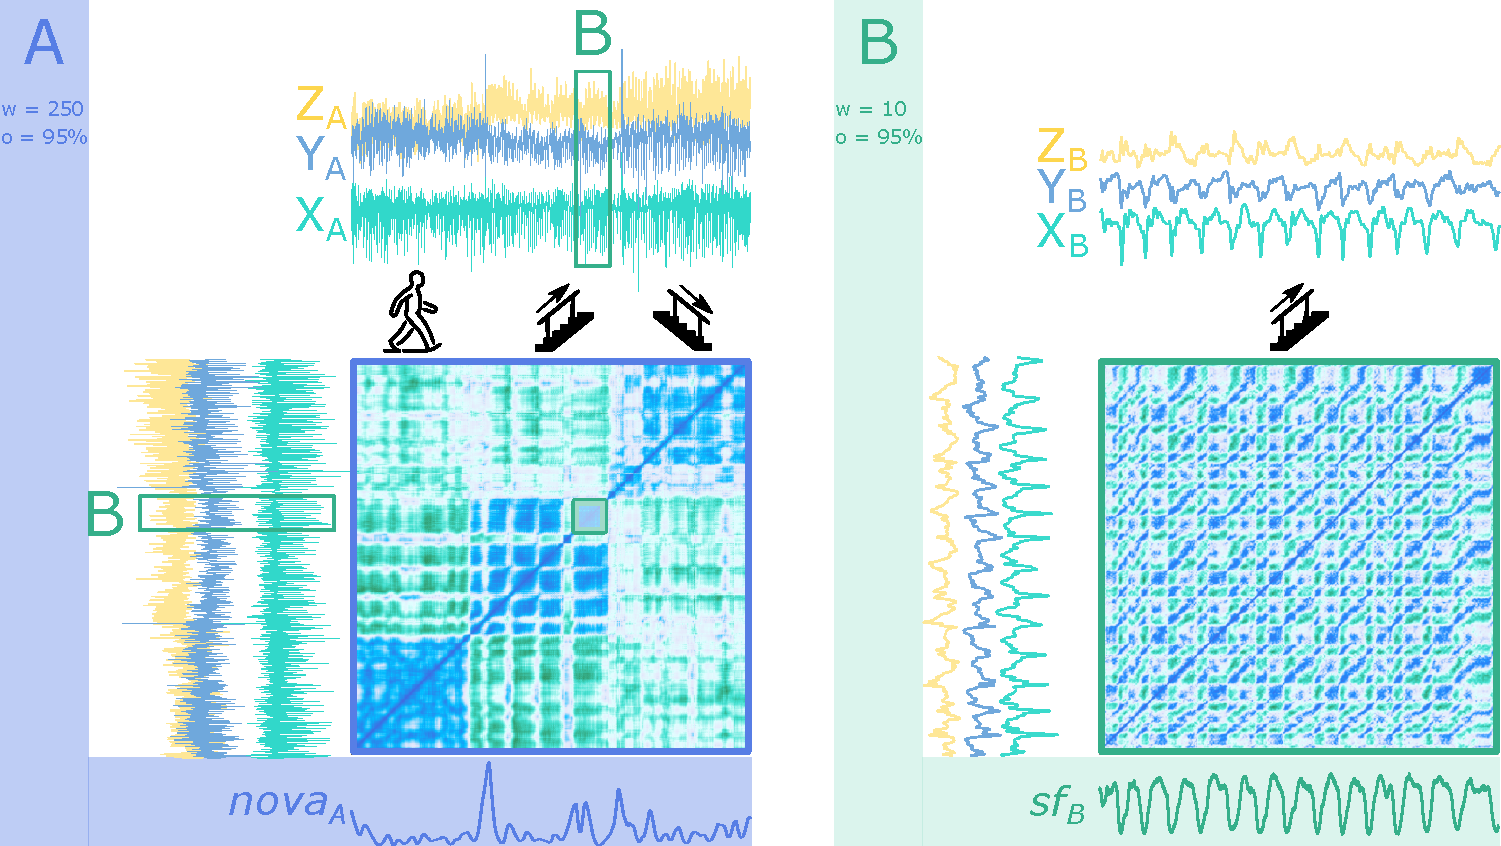
\includegraphics[width=0.85\textwidth]{use_case1_HAR_zoom_in.pdf}     
    \end{subfigure}
    \caption{An \gls{ssm}-based novelty search strategy to detect segmentation events on a signal piece from Dataset 3 (see Section \ref{dat:dataset3}). Top: $window_{size}$=250 samples, $kernel_{size}$=45 samples, and overlap=95\% on the activity sequence Standing $\xrightarrow[]{}$ Laying $\xrightarrow[]{}$ Walking $\xrightarrow[]{}$ Upstairs $\xrightarrow[]{}$ Downstairs $\xrightarrow[]{}$ Sitting $\xrightarrow[]{}$ Standing $\xrightarrow[]{}$ Laying $\xrightarrow[]{}$ Walking $\xrightarrow[]{}$ Upstairs
    $\xrightarrow[]{}$ Downstairs $\xrightarrow[]{}$ Sitting $\xrightarrow[]{}$ Standing
    $\xrightarrow[]{}$ Laying; bottom left: signal change point detection on segment $A$ with a size of 5000 samples, an overlap of 75\%, and a kernel size of 25 samples; bottom right: further zooming in with a window size of 10 samples and an overlap of 95\%, to reveal more periodic details of segment $B$.}
    \label{fig:use_case1}
\end{figure}


Figure \ref{fig:use_case1}(top) exemplifies the \gls{ssm}'s usage on a record of an \gls{har} dataset (\textit{HAR1}, see Section \ref{dat:dataset3}), where the data of all three accelerometer axes is applied. The \gls{ssm} was computed using a 250-sample window size, and a 95\% overlap. Along the diagonal, the novelty function generates block-wise references for estimating activity transition using a 45-sample kernel.

We can identify in Figure \ref{fig:use_case1}(top) that the detected segmentation points match the activity transitions. Although all transitions are visible on the novelty function, the transitions between similar activity patterns in the walking category (straightforward, upstairs, and downstairs) are more challenging to differentiate, as block $A$ suggests, which is plausible since the properties of these segments are morphologically similar.

The proposed unsupervised method automatically and sensitively detects any significant change in properties. As can be found in the yellow-marked part in Figure \ref{fig:use_case1}(top), the period in which the subject was performing the \textit{Upstairs} activity is affected by other changes in the time series. These are significant and also correspond to \textit{block} transitions, which are also evident in the novelty function. 

When \textit{zooming} the \gls{ssm} into segment \textit{A} in Figure \ref{fig:use_case1}(top), the three activities in the walking category can be effortlessly segmented based on the change points revealed by chequerboard patterns, as the two most prominent peaks in he corresponding novelty function pinpoint (see Figure \ref{fig:use_case1}(bottom left)). In addition, it is noticeable that the matrix segments related to \textit{Upstairs/Downstairs} are also segmentable into smaller \textit{blocks}.
As the information is not available in the dataset description, we believe they are a flight of stairs.

Questions may arise at this point. Why is the signal periodicity of the three walking activities not evident in Figure \ref{fig:use_case1}(bottom left)? The reason is that the window size used to compute the \gls{ssm} is relatively large. If features are extracted with a smaller window size closer to the walking period, the \textit{paths} delineating the pattern recurrence will be visible. Figure \ref{fig:use_case1}(bottom right) shows the \gls{ssm} built from segment \textit{B} of the original time series, with a window size of 10 samples and an overlap of 95\%. The \textit{paths} in the matrix enable the periodicity detection with the similarity function $sf_B$.

\subsection{Arterial Blood Pressure (ABP) Signals in Posture Recognition domain}
\label{sec:abp_example}

\begin{figure}
    \centering
    \begin{subfigure}[b]{\textwidth}
         \centering
         \includegraphics[width=0.9\textwidth]{5_abp_example_1.pdf}
    \end{subfigure}\\
    \vspace{5mm}
    \begin{subfigure}[b]{\textwidth}
         \centering
         \includegraphics[width=0.9\textwidth]{5_abp_example_2.pdf}
    \end{subfigure}
    \caption{Novelty search on an \gls{abp} signal from Dataset 5 (\textit{TILT}, see Section \ref{sec:dataset2}). Top: a window size of 5,000 samples, an overlap of 95\%, and a kernel size of 200 samples. The trapezoidal and the square wave mark the ground truth of slow and fast postural transitions. Bottom: the first 10,000 samples, with a window size of 250 samples, an overlap of 95\%, and a kernel size of 200 samples. The right parts of the top and bottom subfigures plot the corresponding similarity profiles for each subsequence segmented by the novelty function.}
    \label{fig:use_case2}
\end{figure}

Many biomedical signals, such as \gls{ecg}, \gls{abp}, and \gls{resp}, contain retrievable structural information like periodicities. Meanwhile, unexpected changes may occur during the acquisition due to physiological responses, medical disorders, or sensing problems like noise, interferences, artefacts, and electrode detachment. We visualize two examples of physiological changes in different types of periodic signals.

The \gls{abp} signal can vary due to postural changes, as an available experiment at \textit{Physionet} confirms \cite{tilt, PhBank}. Figure \ref{fig:use_case2}(top) shows the process of segmenting the \gls{abp} signal based on postural changes, where the trapezoidal and the square wave tag the ground truth of slow and fast postural transitions. The proposed strategy well perceives the change points. Observably, the shape of the raw \gls{abp} signal in each regime is undistinguishable through the naked eye. Therefore, it is constructive to rely solely on the signal itself to implement postural change detection. It is important to point out that the periodicity of the signal is not visible on the matrix because the features were extracted with a window size of 5,000 samples, which is much larger than the period size. A smaller window size of 250 samples in the current scenario allows periodic segmentation, as Figure \ref{fig:use_case2}(bottom) illustrates, where the \gls{ssm} is computed on the first 10,000 samples of Dataset 2 (\textit{TILT}, see Section \ref{sec:dataset2}).
The resulting \textit{similarity} function gives prominence to the periodic nature of the \gls{abp} signal.

The \gls{ssm} of Figure \ref{fig:use_case2}(top) also shows which segments are similar to each other. The blue-coloured parts in the matrix indicate high similarity, presenting that segments from the same posture are more similar than between different postures. For further illustrative purposes, we computed the similarity profiles of each segment as if segmented by the \textit{novelty} function, which evidences that the corresponding sections could be well clustered based on the similarity profiles ($P_A = P_C$ and $P_B=P_D$). In the same way, the similarity profiles in Figure \ref{fig:use_case2}(bottom) examine the similarity between segmented \textit{subsequences}. Profiles with a similar shape can be grouped ($P_A=P_C=P_E=P_G$ and $P_B=P_D$), which can be applied to automatic clustering, as will be exhibited further in the next Section.

\subsection{Electrocardiography (ECG) Signals in Biomedical Domain}
\label{sec:ecg_example}

\begin{figure}
    \centering
    \includegraphics[width=0.9\linewidth]{5_ecg_example.pdf}
    \caption{An \gls{ecg} signal with a \textit{pulsus paradoxus} condition starting at the $10,000^{th}$ sample from Dataset 6 (see Section \ref{dat:dataset15}). Left: the \gls{ssm} diagnoses two modes in the signal, whose patterns are zoomed in the circle thumbnails, respectively; right: zooming parts of the original signal can verify \gls{ssm}'s ability of automatic \gls{ecg} pattern change detection and contribution to segmentation.}
    \label{fig:use_case3}
\end{figure}

Another widely used biomedical signal, \gls{ecg}, also testifies to the feasibility of our proposed method. The \gls{ecg} signal in Figure \ref{fig:use_case3}(left) displays the presence of the condition called \textit{pulsus paradoxus}, an exaggerated fall (>10 mmHg) in the subject's blood pressure during inspiration \cite{pulsusparadoxus2}, which can also occur when the patient changes sleeping posture after heart surgery\cite{eamonn_segmentation}, as the following example relates. Similar to the \gls{abp} signal elucidated in Section \ref{dat:dataset2}, the human eye hardly perceives the change points in \gls{ecg} signals. Once again, our proposed strategy shows strength.

In addition to the novelty detection, segment \textbf{\textit{A}} previous to the pulsus paradoxus occurrence can be partially detailed again to reveal minor changes due to additional noise, verifying \gls{ssm}'s sensitivity to structural changes, as Figure \ref{fig:use_case3} (right) imparts.

\subsection{Single Channel versus Multidimensionality Application in Multi-Sensor Scenarios}
\label{sec:multi_example}

The proposed method accepts both single- and multidimensional records. The difference regards the number of features extracted. As compared in Figure \ref{fig:use_case4}, the same set of features is extracted from each time series to build the $F_M$.
Using a single or several time series of a multidimensional record is an option, depending on the purpose. In some cases, the use of non-complete dimensions may miss relevant events, as Figure \ref{fig:use_case4} instances the record ``Occupancy'' from Dataset 9 (\textit{ATCPD}, see Section \ref{dat:dataset10}). 

The record is a multidimensional time series that measures room occupancy based on temperature, humidity, light, and $CO_2$. By comparing the signals and formations in the left and the right parts of Figure \ref{fig:use_case4}, it can be understood that some events can be detected using the $CO_2$ series exclusively, but some are missed.

\begin{figure}
    \centering
    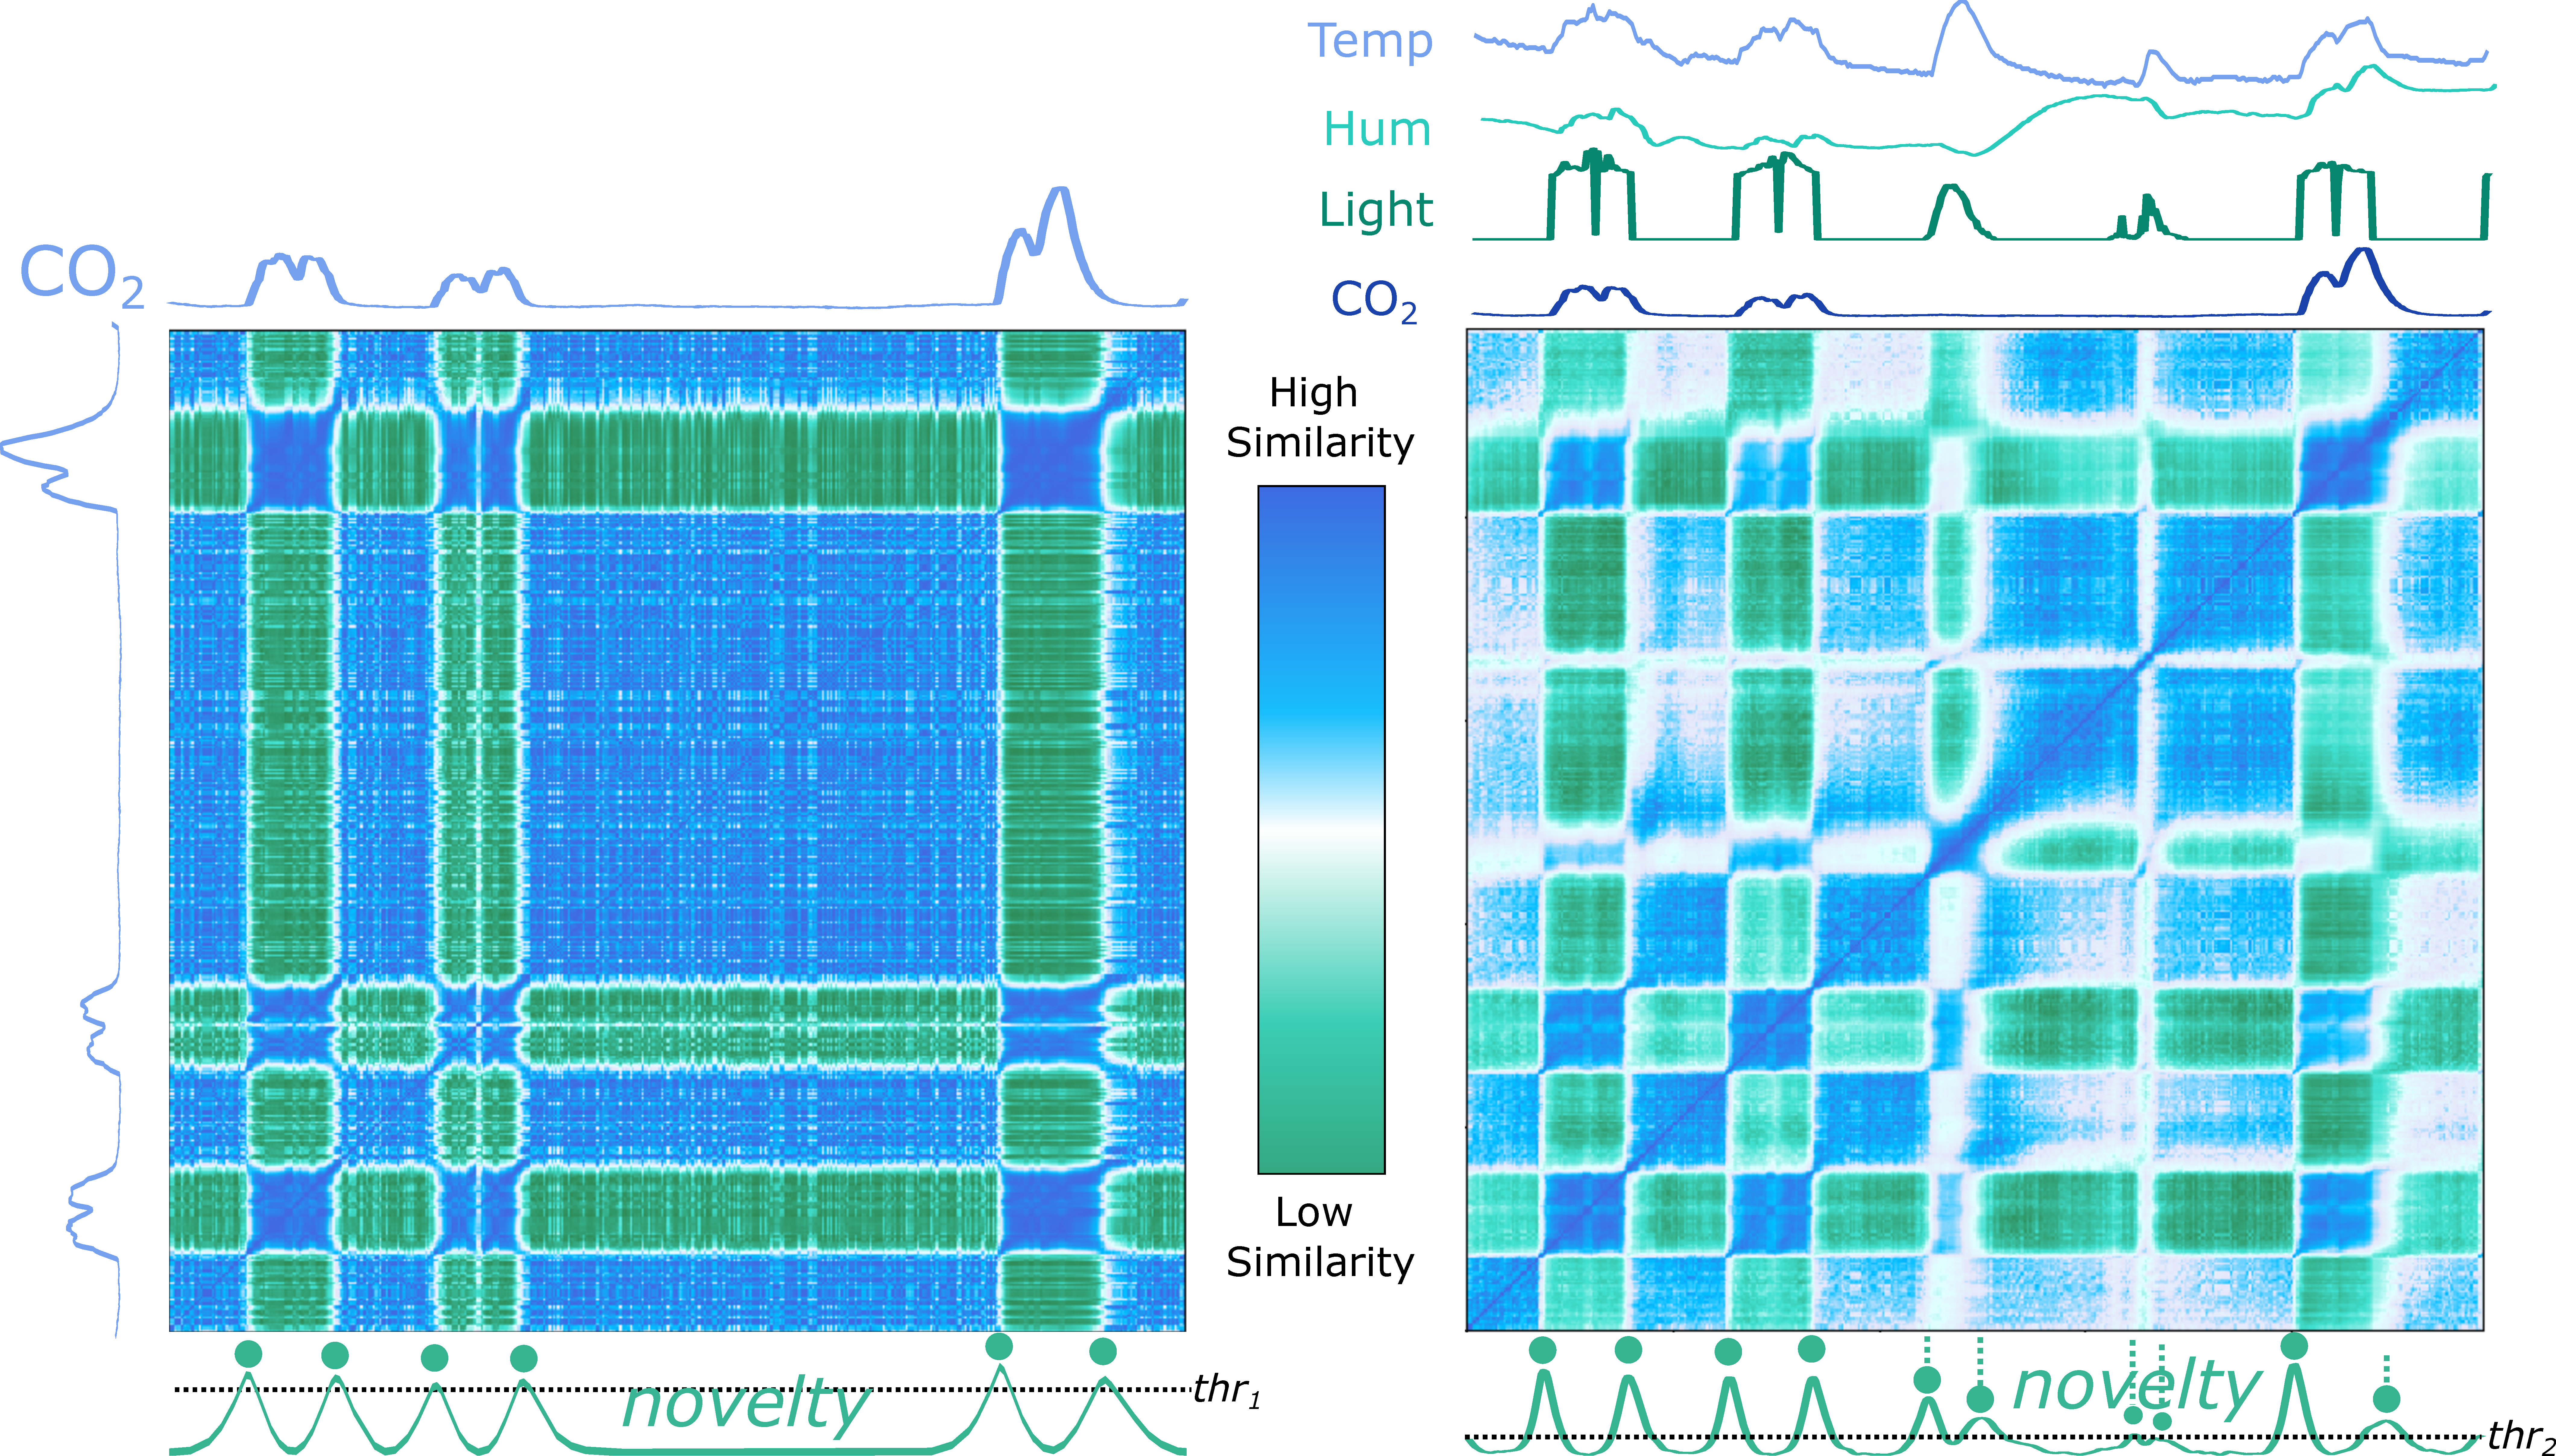
\includegraphics[width=\textwidth]{use_case4_multi.pdf}
    \caption{The proposed method applied on the \textit{Occupancy} record of Dataset 9 (\textit{ATCPD}, see Section \ref{dat:dataset10}). Left: calculations on the separate $CO_2$ time series only; right: calculations performed by extracting features on the complete four time series.}
    \label{fig:use_case4}
\end{figure}

\section{Time Series Summarization}

The aforementioned examples show how the proposed method can be used as a strong and reliable visual tool. It is possible to see how a time series is structured, how similar are segments, and if these are periodic or not. The information available is relevant to support the labeling process of the analyst, but it also can be used to summarize a time series and give a meaningful report about it. 
\par
Following the presented work, we studied how to use it for a meaningful summary of time series. This process is inspired by methodologies that exist in other scenarios for data summarization techniques with statistical analysis, such as the available methods from the \textit{pandas python library}: \textit{pandas.profile()} and \textit{pandas.describe()}. These methods can provide a summarization of a dataset (typically of categorical data) that is given as input. A similar method is not known for time series. In order to develop such a method, we should first understand what is meaningful and relevant to represent as a summary.

\subsection{Elements with Relevance}

In this section, we have been discussing which elements are relevant in time series, mostly associated with \textit{events}. From \textit{events} we can segment homogeneous \textit{subsequences}, recurrent or periodic patterns and anomalies. The relationship between these segments is possible by analysing their similarity. In addition, a characterization of the segments is possible with statistical analysis. In that sense, the relevant elements to summarize in a time series are (1) \textit{homogeneous segments}, (2) \textit{periodic patterns}, (3) \textit{recurrent patterns}, (4) \textit{anomalies}, (5) association based on similarity and (6) statistical characterization.

\subsection{Compact Design}

Strategies that are typically used to present information compactly are found in several domains. In text analysis, for instance, the relationship between repeating sequences is illustrated with arc diagrams \cite{bitmap, arcplots}. These show where repeating sequences occur in a very concise way. This has a range of applications that include, for example, text and \textit{DNA} sequence analysis. For instance, graphical genome maps are found to concatenate a significant amount of information in a very compact way. Genome features and sequence characteristics are assessed with this visual strategy. An example can be found in Figure \ref{fig:genomic2} (see Section \ref{sec:literature_summarize}). This type of visualization inspired the summarization approach proposed for time series.
\par
The proposed visualization strategy has several elements that can be used to transform the \gls{ssm} into a compact form of filtered information. The elements are  illustrated in Figure \ref{fig:summarize_steps} and listed as follows:
\begin{itemize}
	\item Novelty ($N$) and Subsegment Layers ($P$) - The novelty layer $N$ has the segments resulting from the novelty segmentation step, color-coded based on how similar each \textit{subsequence} is with the first segment. The subsegment layer $P$ partitions each novelty segment into single periods, when the \textit{subsequence} is periodic;
	\item \textit{Chords} ($C$) - Each novelty segment is connected to the most similar subsegment with a colored connector;
	\item Signal Layer - The original signal is located on top of the partitioned segments.
\end{itemize}


\subsection{A step-by-step example}

\begin{figure}
\centering
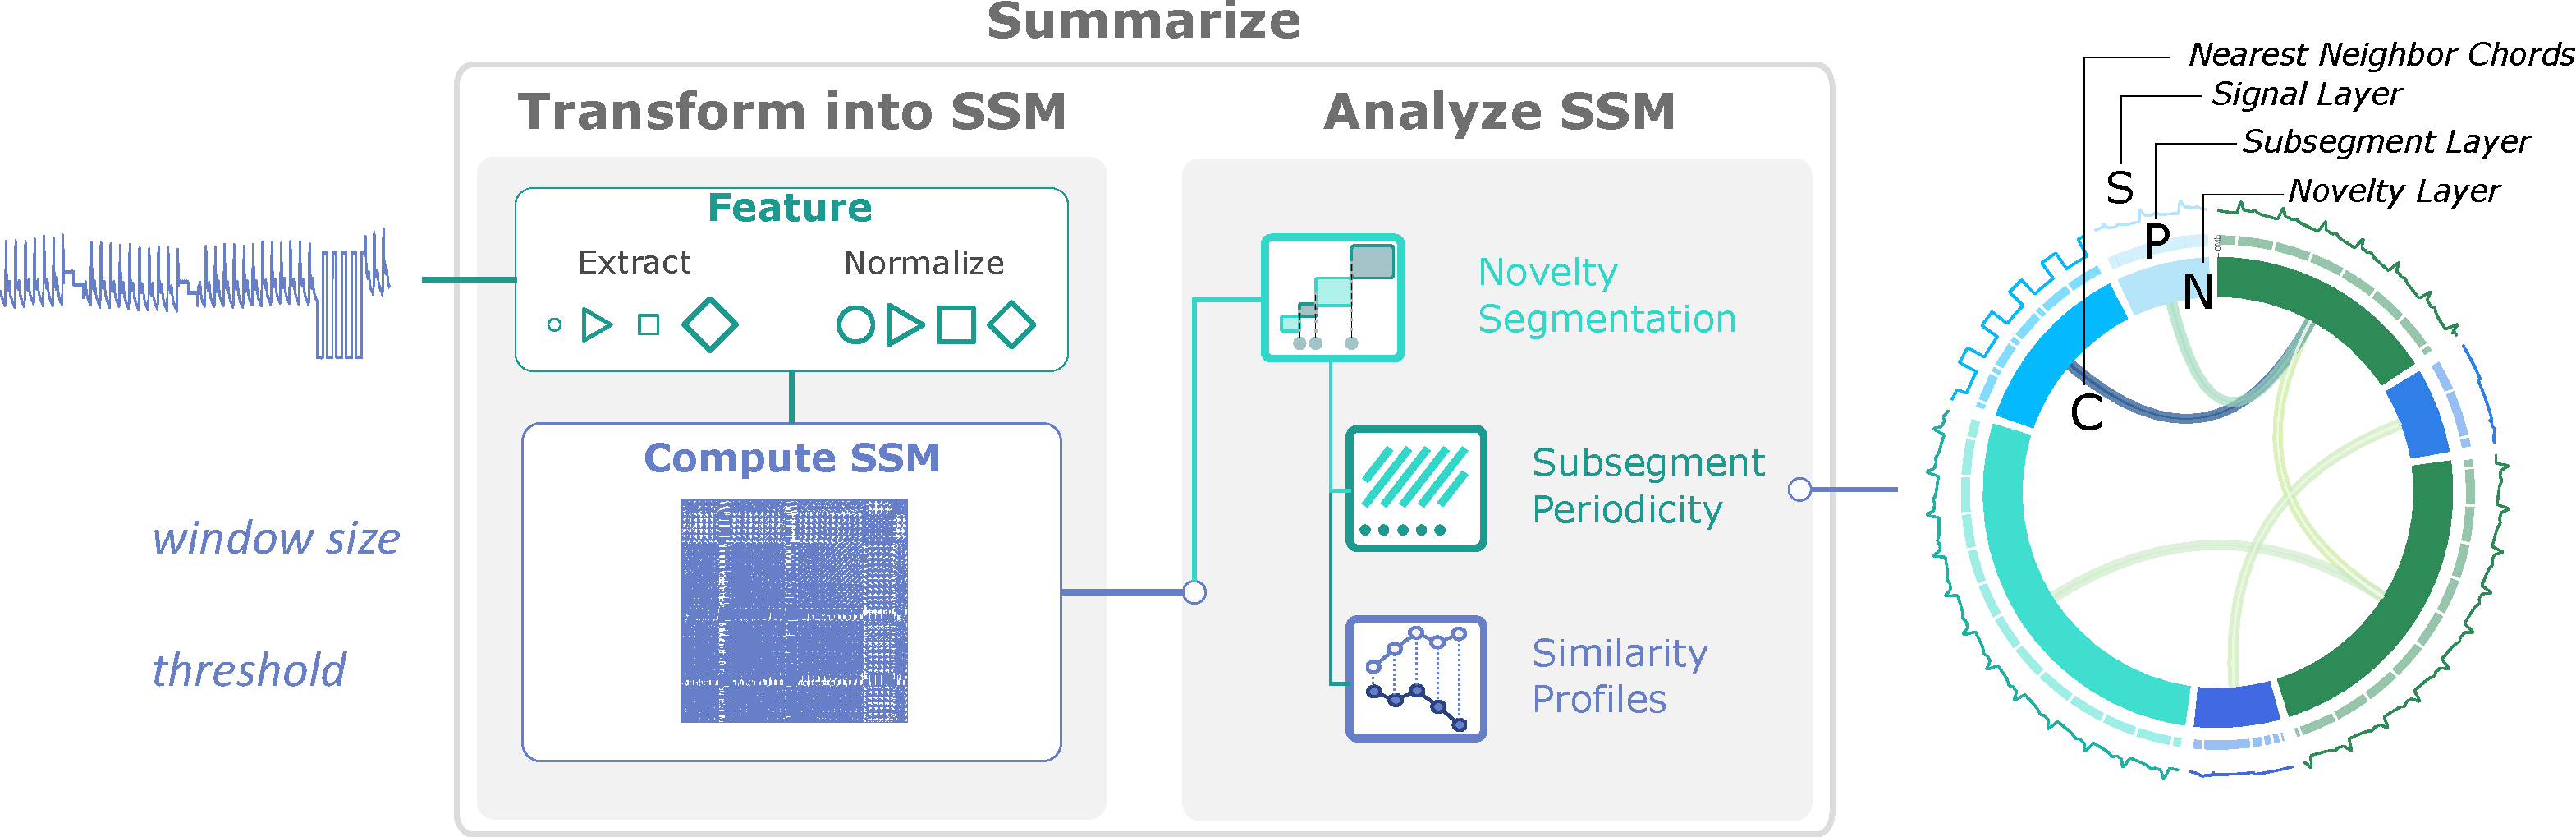
\includegraphics[width=\linewidth]{summarize_steps.pdf}
\caption{Steps to use the aforementioned methods on the \gls{ssm} to summarize the time series into a circular plot with C - chords that connect nearest neighbors, S - the signal layer, P - the subseqment layer and N - the color coded novelty layer. Each of these elements of the summarized plots are built based on novelty segmentation, subsegment periodicity check and similarity profiles.}
\label{fig:summarize_steps}
\end{figure}

The steps are indicated in Figure \ref{fig:summarize_steps} for the \gls{abp} signal example. After computing the \gls{ssm}, it is firstly analysed to segment the signal based on the \textit{nova} function. These segments are then compared based on the \textit{similarity profiles}. Additional layers can be created by performing an iterative and multi-scale segmentation. With this process, the time series is segmented (\textit{novelty layer}), subsegmented (\textit{subsegment layer}), each segment is connected to the nearest neighbor segment (\textit{nearest neighbor chords}) and the colors for each segment is given based on their similarity to the first segment. Figures \ref{fig:summarize_step1}, \ref{fig:summarize_step2} and \ref{fig:summarize_step3} show the step-by-step process to summarize the time series by analysing the \gls{ssm}. 

\begin{figure}
\centering
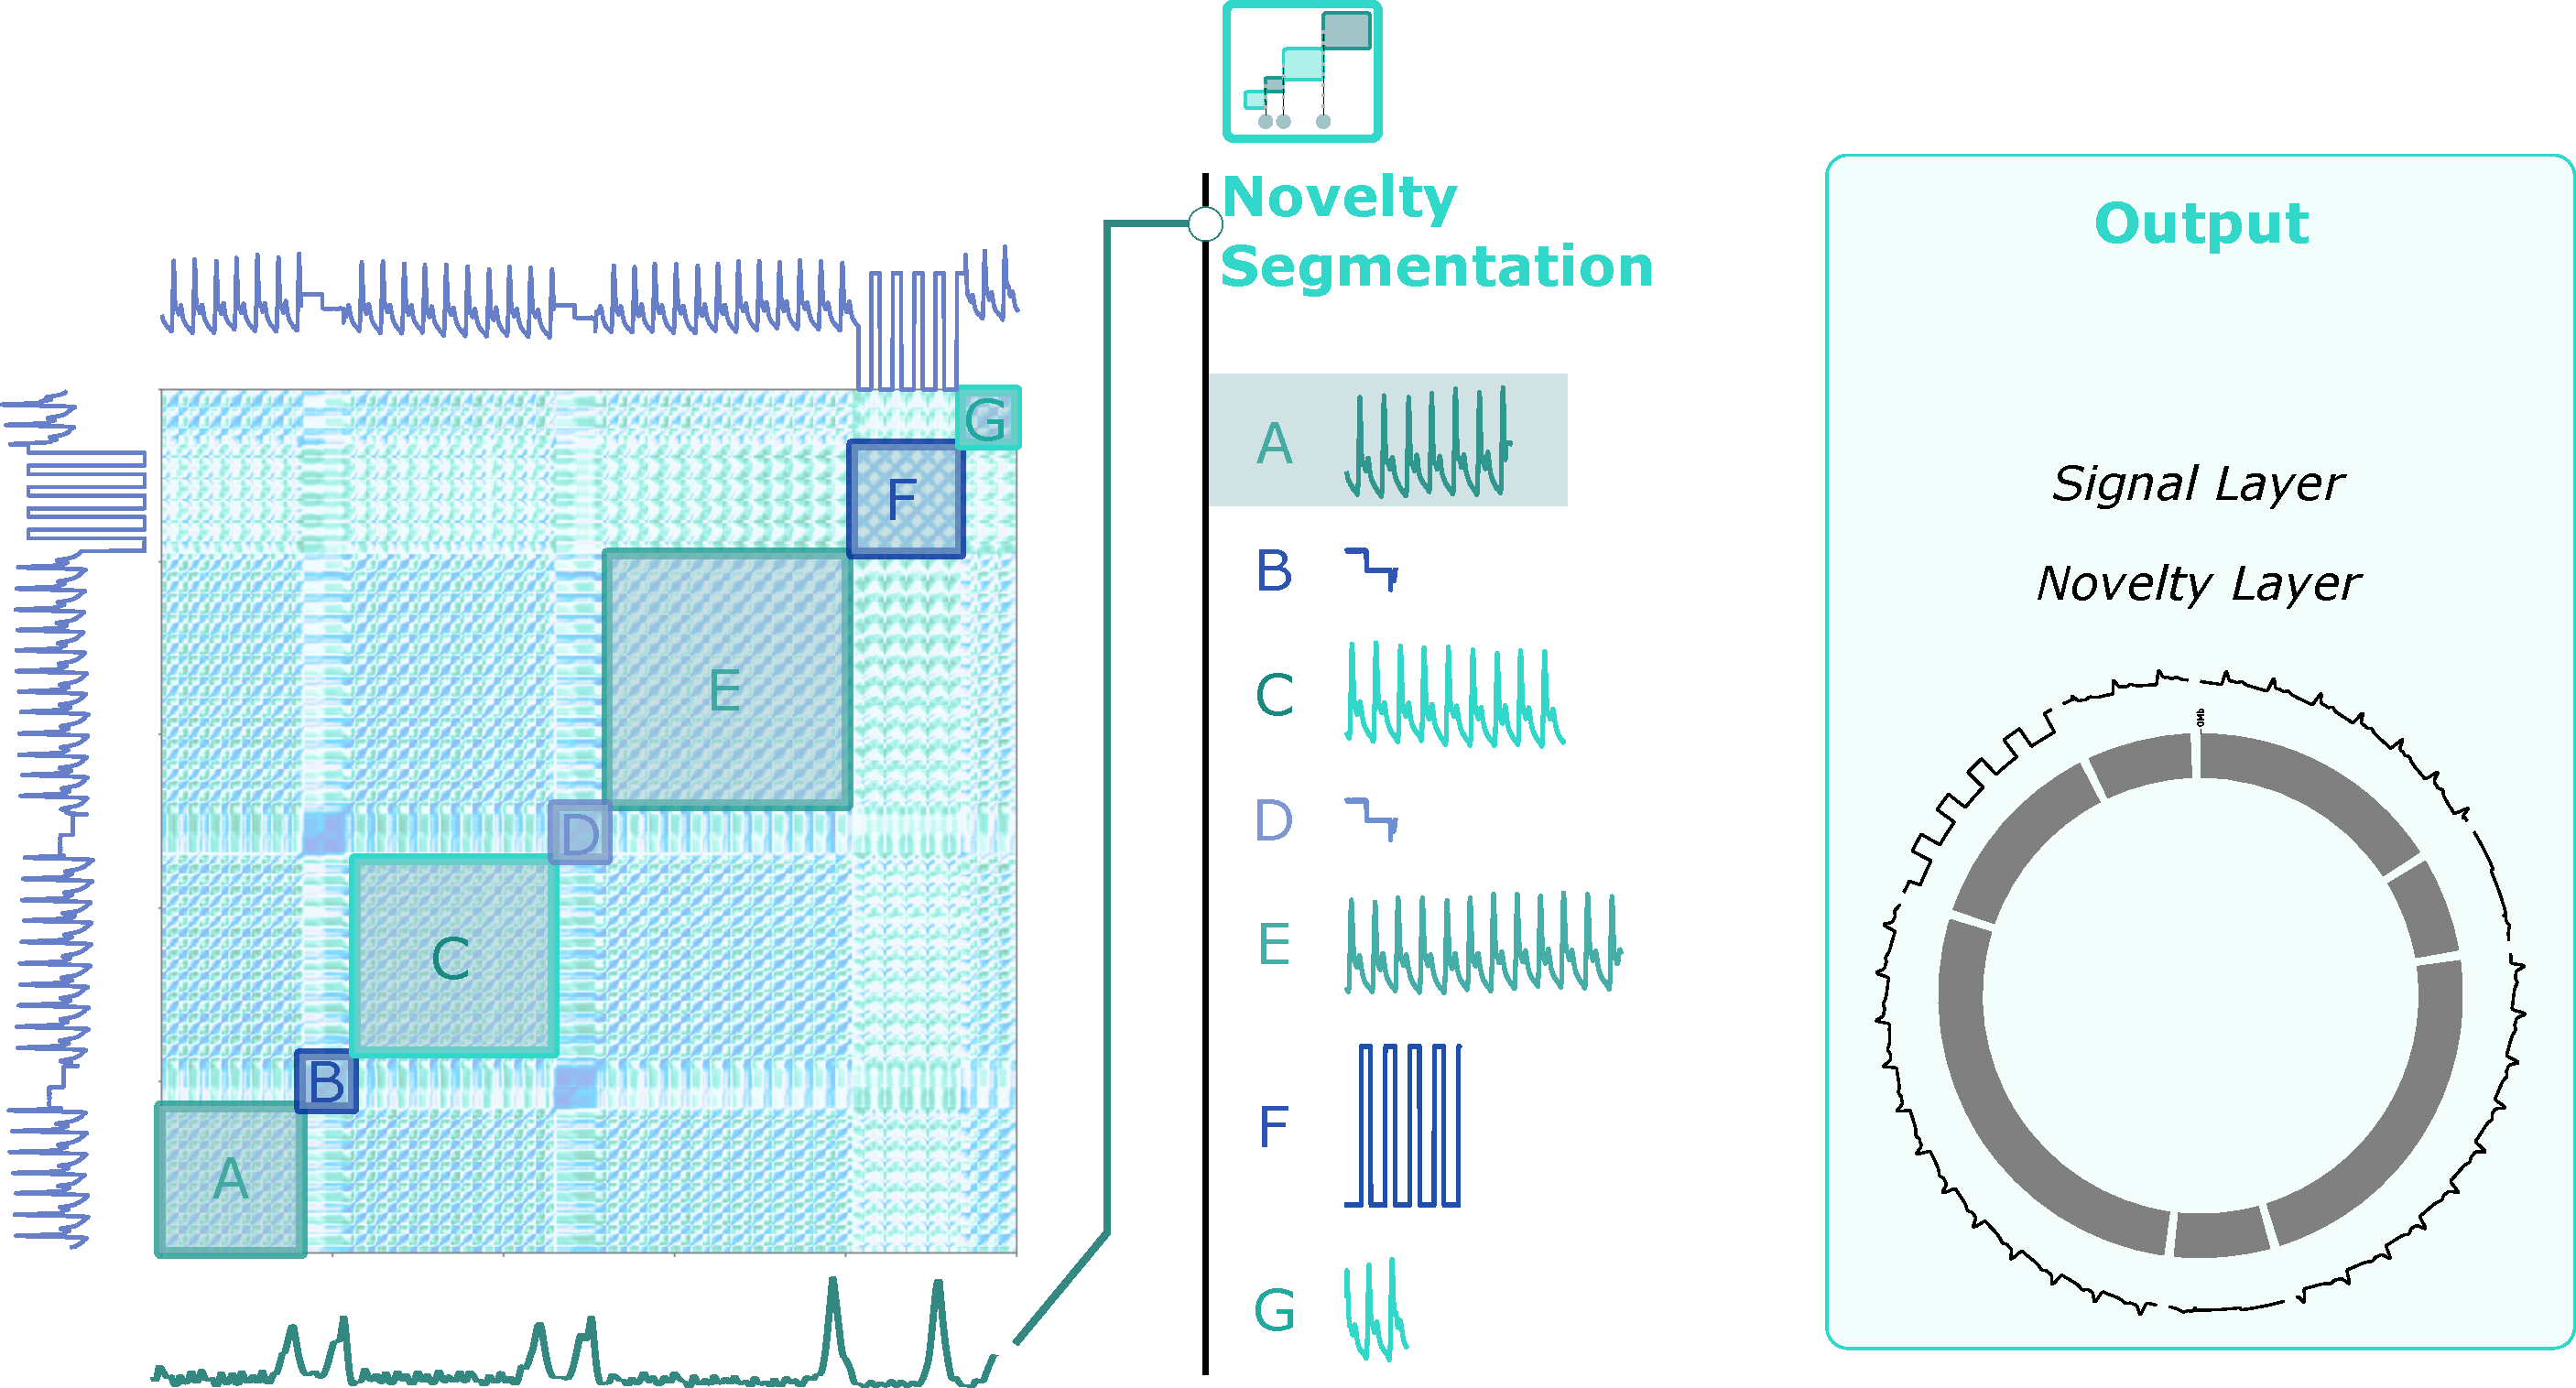
\includegraphics[width=0.85\linewidth]{summarize_step1.pdf}
\caption{How to reach a standard format. This step applies the novelty search method to find the segmentation points. The signal is broken into A to G segments.}
\label{fig:summarize_step1}
\end{figure}

The \textit{nova} function segments the time series into seven segments. The reader can notice that segments A, C, E, and G are similar and separated by segments B, C and F, represented by a failure in the connection of the sensor. From this first segmentation, the \textit{novelty layer} is created, indicating how structured is the signal, as presented in Figure \ref{fig:summarize_step1}.

\begin{figure}
\centering
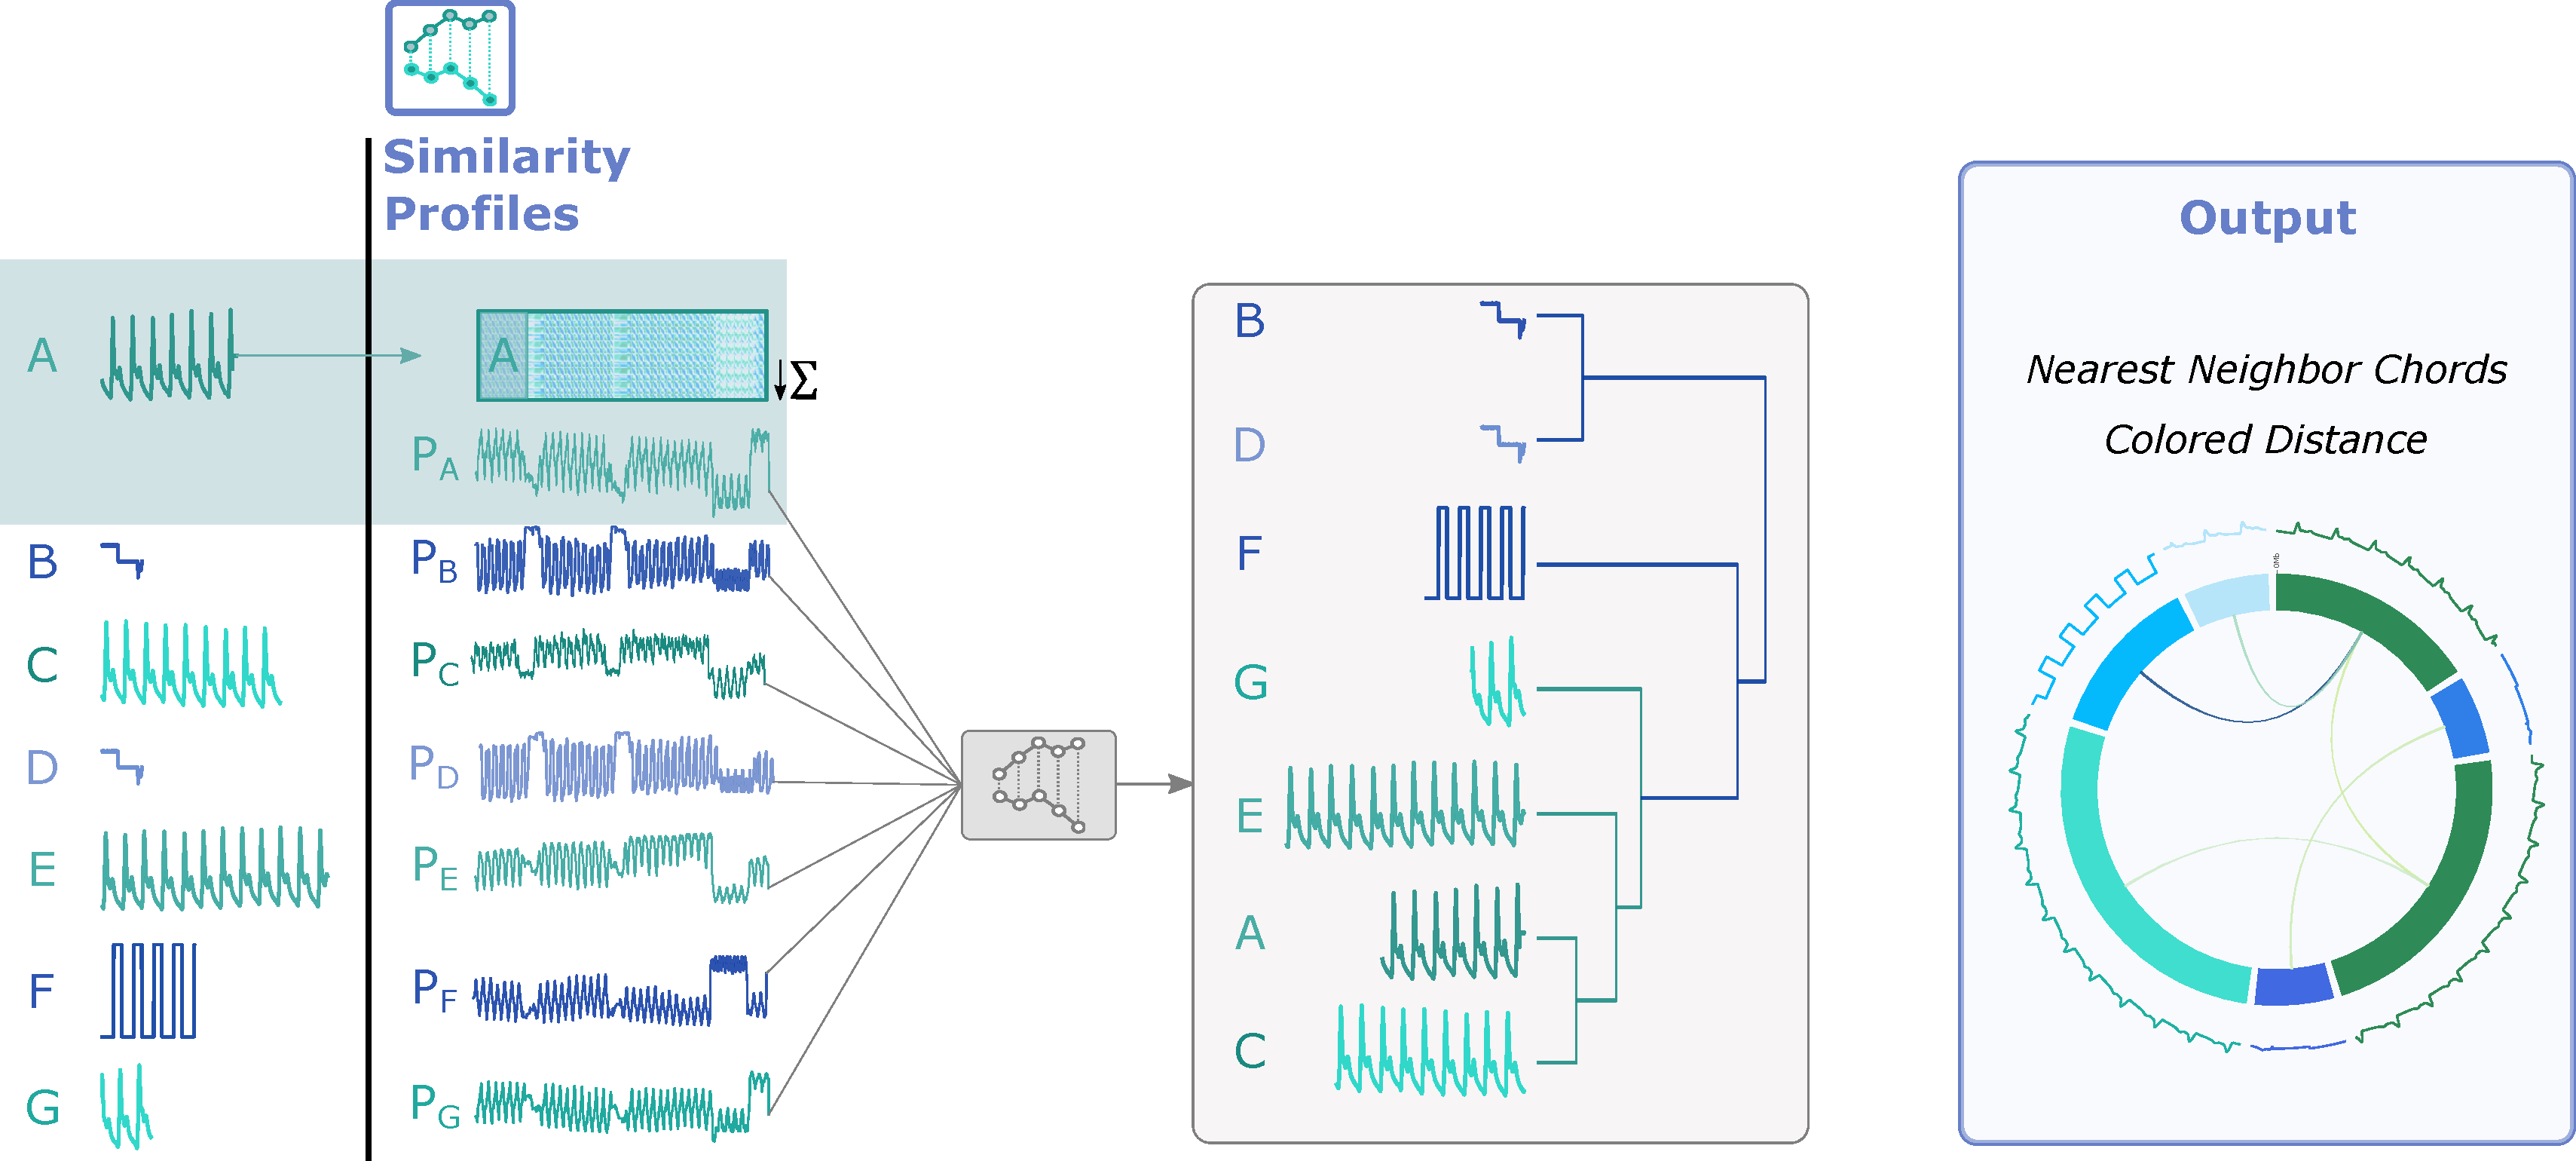
\includegraphics[width=\linewidth]{summarize_step2.pdf}
\caption{From each segment, a similarity profile can be computed. The pairwise euclidean distance is applied to these profiles, from which a dendogram is created. From this association, layer C can be drawn and the colors of the novelty layer can be added. Segment A is highlighted for the next step.}
\label{fig:summarize_step2}
\end{figure}

Further, the segments are compared with the \textit{similarity profiles} of each segment. Figure \ref{fig:summarize_step2} illustrates as example the rows of the \gls{ssm} delimited by segment A and the column-wise average into $P_A$. The same process is applied to each segment. From this Figure, the reader may notice that the profiles $P_A$, $P_C$, $P_E$, and $P_G$ are more similar, while profiles $P_B$ and $P_D$ are more similar as well. The pairwise distance is computed between profiles, which can then be used to extract the nearest neighbor of each segment, as well as transform the distance values between segments into color. 
\par
The pairwise distance between profiles is also used to illustrate how the segments are ordered and clustered by the dendrogram of Figure \ref{fig:summarize_step2}. The dendrogram shows that there are three main clusters, being cluster one represented by segments A, C, E, and G; the second cluster has segment F and the third cluster groups segments B and D. It is important to note that typical distance measures, such as the \gls{ed} or \gls{dtw}, would not be able to directly sort these segments correctly. Using \textit{similarity profiles} is more robust and invariant to the size and time distortions. The illustrated dendogram also has distance measures between the novelty segments. We use the distance from each segment to the first segment ($A$) and select the corresponding color-code to be represented on the summarized layout. 

\begin{figure}
\centering
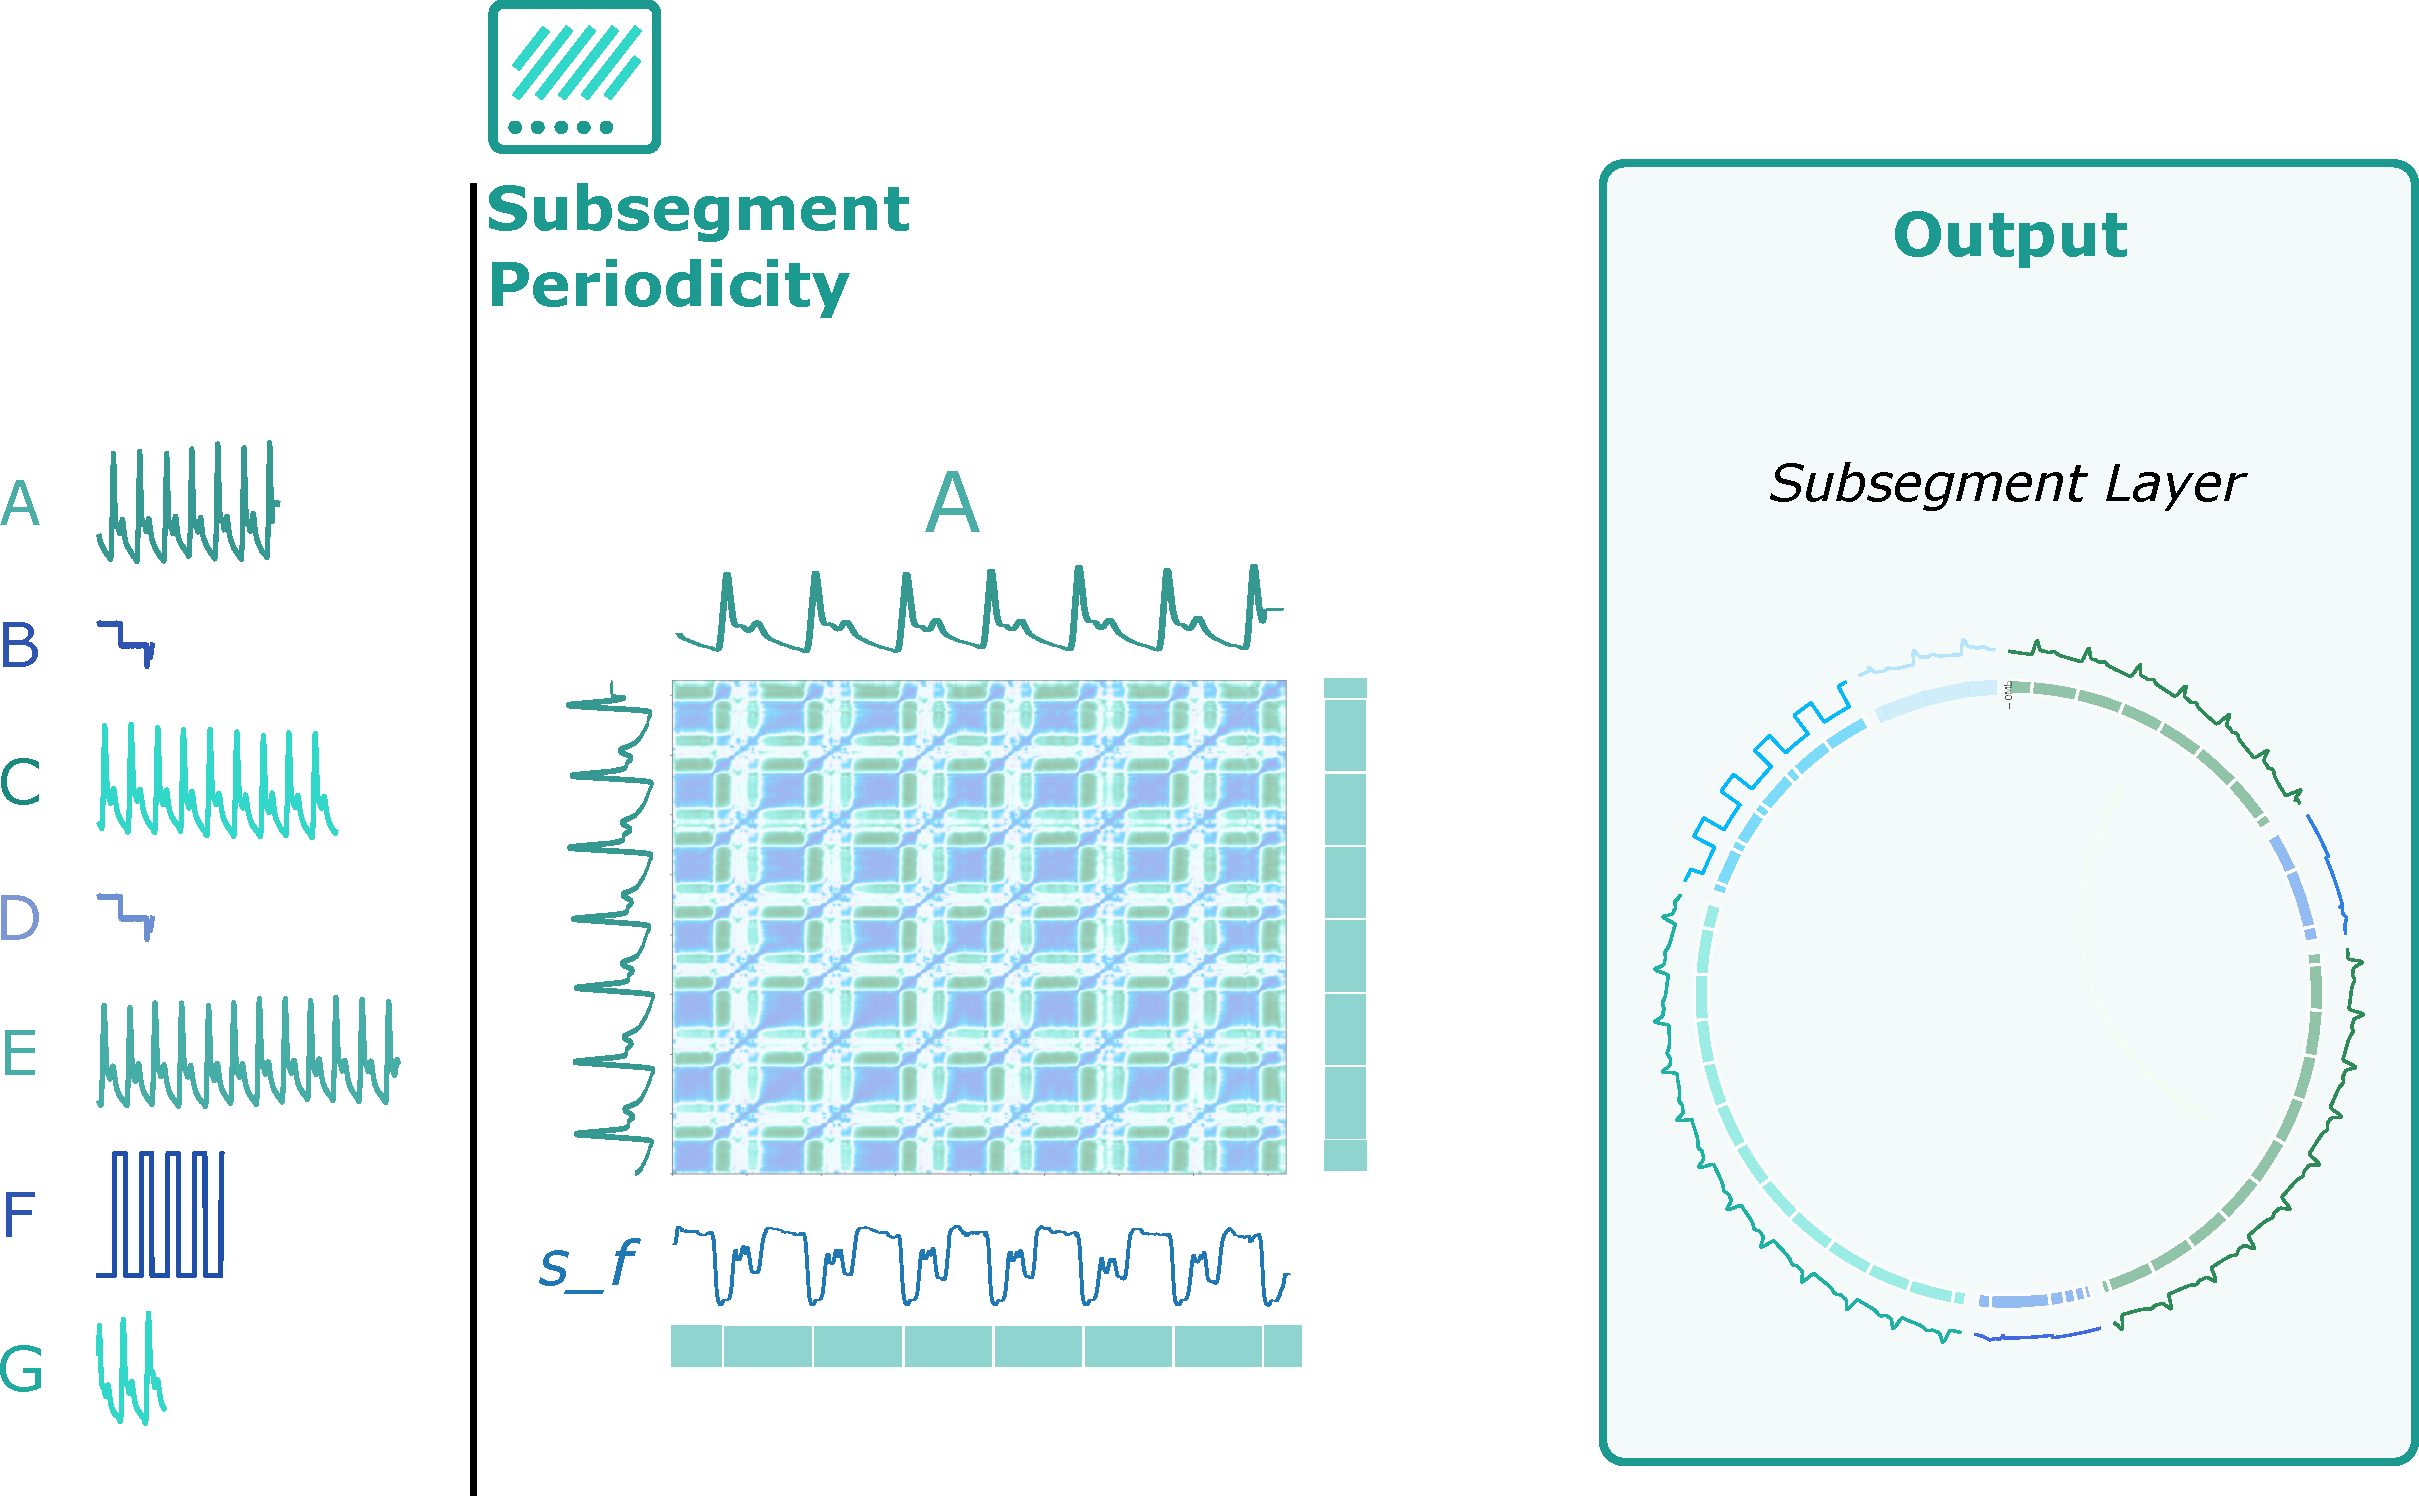
\includegraphics[width=0.75\linewidth]{summarize_step3.pdf}
\caption{After finding the first layer of the segmentation points, the periodicity of each segment can be checked and added as a sublayer of segments, adding layer P. In this case, segment A is the example.}
\label{fig:summarize_step3}
\end{figure}

Finally, the process to summarize the time series can be iterative by adding \textit{subsegment layers}. These layers can be added by performing the \textit{novelty search} on the previously segmented time series with a smaller time scale or segmenting the time series based on periodicity. In this case, the signal is periodic, therefore Figure \ref{fig:summarize_step3} illustrates the \textit{periodic search}, where periods are segmented by the minima of the $s_f$.
\par
This summarization process is mostly graphical and follows the results of each process for information retrieval from the \gls{ssm}. Therefore, this method will not present overall results or be validated in Chapter \ref{cha:results}.
